\chapter{The MMSODA Toolbox for MATLAB}
\label{ch:mmsoda}

There are various softwares that implement the Master-Worker paradigm. The most commonly used Master-Worker software is probably MPI\index{Message Passing Interface}\index{MPI}, which stands for \textit{Message Passing Interface}. Most cluster computers have some form of MPI installed. We will use the GNU version of OpenMPI\index{MPI!OpenMPI/GNU}\index{OpenMPI/GNU}, since this is the default MPI package at the LISA cluster computer.

We have developed a parallel MATLAB version of SODA \citep[e.g.][]{vrug-diks-gupt-bout-vers-2005} that makes use of MPI. The software package is called `The MMSODA Toolbox for MATLAB', or MMSODA for short (MMSODA stands for MATLAB-MPI-SODA). In this chapter, we will look at how to set it up.

MMSODA offers the functionality of a number of previously separate softwares, namely SCEM-UA \citep{vrug-gupt-bout-soro-2003}, SODA \citep{vrug-diks-gupt-bout-vers-2005,vrug-robi-vess-2005,clar-vrug-2006}, MOSCEM-UA \citep{vrug-gupt-bast-bout-soro-2003}, multi-objective SODA \citep{vrug-stau-wohl-robi-vess-2008}, the MPITB-parallel version of SCEM-UA implemented in Octave \citep{vrug-onua-robi-bout-dekk-sloo-2006}, and the MPITB-parallel version of SODA implemented in Octave \citep{vrug-gupt-onua-bout-2006}. Additionally, MMSODA offers a parallel version of multi-objective SCEM-UA, and a parallel version of multi-objective SODA, both of which did not exist previously. Moreover, MMSODA does not use Octave when running in parallel, because Octave does not evaluate code as quickly as does MATLAB. MMSODA circumvents (in a legal fashion) the license requirements that are often an impediment to parallel computation by compiling the MATLAB code into a binary which can be run without any license. Compiling the binary, however, does require a license, both for the MATLAB program itself, as well as for the MATLAB Compiler Runtime Toolbox. Fortunately, the required licenses are available on most cluster environments targeting a scientific and engineering audience.

In short, the acronyms mentioned above mean that: MMSODA can do parameter tuning with or without intermediate state updating by an ensemble Kalman Filter; that MMSODA supports both single-objective and multi-objective optimization; and that the optimization can be run either sequentially on a local machine, or in parallel on a cluster computer.

The serial/parallel capability is particularly attractive, since it allows the users to set up their optimizations locally on their own machines, thus ensuring a familiar development environment without the need to make the code compatible with Octave syntax. When the user finishes setting up the optimization, running it on a cluster computer is simply a matter of copying the relevant directory to the cluster storage using standard tools (e.g. WinSCP) and compiling the software by executing a script that comes with the software. Furthermore, MMSODA is fully documented with HTML documentation which can be accessed in the same way as MATLAB's built-in commands, namely through the \texttt{doc} command.

The remainder of this chapter explains how to set up increasingly sophisticated optimizations within the MMSODA framework. Let's start off with a single-objective SCEM-UA optimization of a benchmark function \texttt{calcLikelihood()}, and let's not do anything in parallel just yet.

\section{MMSODA in `bypass' mode; sequential execution}

\smallq{You should have received `esibayes.zip' with this document. Unzip it into a directory on your local machine.}

As you can see, the `esibayes' directory contains a number of subdirectories. Among these, the `mmsoda-toolbox' directory is probably the most important: it contains the MATLAB toolbox that this chapter is about. Most of the other directories have names like `soda-so-something' or `bypass-mo-something'. The specific meaning of these names will become clear later; for now, it suffices to say that they are example projects of how to use the MMSODA toolbox for MATLAB with different models and different configurations. Finally there are two more directories, one labeled `template-project', and one labeled `other'. The former contains a rudimentary structure of an MMSODA project, whereas the latter contains some files that we will be using later on.

\smallq{Let's get started by making a new directory next to the \texttt{mmsoda-toolbox} directory. Let's call this directory \texttt{example1}. Change directory into \texttt{example1}, and create three directories in it called \texttt{data}, \texttt{model}, and \texttt{results}. (We won't always use all three directories, but MMSODA expects all three to be present regardless of whether they are used). So now you have a directory somewhere on your local storage device that has at least the following subdirectories:
\begin{itemize}
\item{\texttt{esibayes/example1}}
\item{\texttt{esibayes/example1/data}}
\item{\texttt{esibayes/example1/model}}
\item{\texttt{esibayes/example1/results}}
\item{\texttt{esibayes/mmsoda-toolbox} (which includes a bunch of subdirectories and subsubdirectories that are not relevant for the moment).}
\end{itemize}
}

\smallq{Open MATLAB and set your working directory to \texttt{example1}.}

\smallq{Before we can use the functionality provided by the MMSODA Toolbox for MATLAB, we need to tell MATLAB about its existence by adding the main directory to the MATLAB search path. You must do this using the \texttt{addpath} command as follows:\\
\texttt{>> addpath(\squote{s})}, in which \texttt{s} indicates the location of the MMSODA directory. For example, it could be:\\
\texttt{>> addpath(\squote{C:\textbackslash{}Users\textbackslash{}jspaaks\textbackslash{}esibayes\textbackslash{}mmsoda-toolbox})}\\ on a Windows machine or \\
\texttt{>> addpath(\squote{/home/jspaaks/esibayes/mmsoda-toolbox})}\\
on Linux.
}
\smallq{At the MATLAB prompt, type:\\
\texttt{>> mmsoda --docinstall}\\
to complete the MMSODA setup. In principle, you only have to run this command once per MATLAB session, as long as you do not change the location of the `mmsoda-toolbox' directory on your storage.}

\smallq{Test whether everything works as it should by typing: \\
\texttt{>> doc mmsoda} \\
at the MATLAB command prompt. This should bring up MATLAB's help browser. Click on the link `View HTML documentation for this function in the help browser'. You should now see an overview of the functions comprising the MMSODA Toolbox for MATLAB.}

\smallq{Spend at least 12 minutes to browse through the documentation. In any case, make sure to read the documentation on `mmsoda.m'.}

The function that we want to maximize implements the double-normal probability distribution:
\begin{equation}\label{eq:double-normal}
\begin{align}
p = \frac{1}{2}\cdot{}\frac{1}{\sqrt{2\pi\sigma_1^2}}\:e^\mathlarger{-\frac{1}{2}\left(\frac{x-\mu_1}{\sigma_1}\right)^2} & +\dots \\
    \frac{1}{2}\cdot{}\frac{1}{\sqrt{2\pi\sigma_2^2}}\:e^\mathlarger{-\frac{1}{2}\left(\frac{x-\mu_2}{\sigma_2}\right)^2} & \\
\end{align}
\end{equation}
with $\mu_1 = -10$, $\sigma_1 = 3$, $\mu_2 = 5$, $\sigma_2 = 1$, respectively. The parameter that is optimized (or, equivalently, whose probability distribution we will estimate by means of the MMSODA Toolbox for MATLAB) is $x$. For example, for $x=4.5$, $p = 0.1760$.

%p=\frac{1}{2}\cdot{}\frac{1}{\sqrt{2\cdot{}\pi\cdot{}\sigma{}_1}}\cdot{}\mathrm{exp}\left[-\frac{1}{2}\cdot{}\left(\frac{x-\mu_1}{\sigma_1} \right)^2 \right] \quad & + \\
%\frac{1}{2}\cdot{}\frac{1}{\sqrt{2\cdot{}\pi\cdot{}\sigma{}_2}}\cdot{}\mathrm{exp}\left[-\frac{1}{2}\cdot{}\left(\frac{x-\mu_2}{\sigma_2} \right)^2 \right] \quad & \\

Because MMSODA expects the objective function to return a log-likelihood $l$, we must actually take the natural logarithm of $p$ as the objective score:
\begin{equation}\label{eq:log-likelihood}
l=\mathrm{ln}\left(p\right)
\end{equation}

\subsection{Creating the `constants.mat' and `conf.mat' files}

Before we actually start writing any code for this objective function however, let's first create the `conf.mat'\index{conf.mat} and `constants.mat'\index{constants.mat} files that are always needed for running \texttt{mmsoda()}.

\smallq{Start a new text file in the MATLAB editor and save it as `makeconf.m'\index{makeconf.m} in the current working directory.}

\smallq{At the first line in `makeconf.m', add the following:\\
\texttt{function makeconf()}\\}

Now we need to edit the contents of `makeconf.m' as follows.

\smallq{At the MATLAB prompt, type \\
\texttt{doc mmsoda} \\
and bring up the HTML documentation for the \texttt{mmsoda()} function.}

Near the bottom of the documentation, there is an overview of the configuration variables that must be specified for a given type of optimization. For our double-normal example, we will use MMSODA in `bypass' mode\index{MMSODA!bypass mode}. This mode is used when the log-likelihood can be estimated directly from the parameter vector, without the need to run a (dynamic) model structure.

\smallq{If you look in the table with the configuration variables, you'll see that only 5 variables are required for running MMSODA in `bypass' mode. These are \texttt{modeStr}, \texttt{objCallStr}, \texttt{parNames}, \texttt{parSpaceHiBound}, and \texttt{parSpaceLoBound}. Make sure you understand the description for each of these.}

\smallq{Return to `makeconf.m' and add the following:\\
\texttt{modeStr = \squote{bypass};}\\
\texttt{objCallStr = \squote{calcLikelihood};}\\
\texttt{parNames = \{\squote{x}\};}\\
\texttt{parSpaceHiBound = [10];}\\
\texttt{parSpaceLoBound = [-30];}\\
}

With the above settings we specify that we want MMSODA to do a bypass run, in which the function `calcLikelihood.m' (which we will create shortly) is optimized. \texttt{calcLikelihood} has one tunable parameter, \texttt{x}. The bounds that we set on the search for the optimal value of \texttt{x} are \texttt{[-30,10]}.

\smallq{At the last line in `makeconf.m', add the following:\\
\texttt{save(\squote{./results/conf.mat})}\\}

\smallq{Save and close `makeconf.m'.}

Next, we need to create `constants.mat' by a similar procedure.

\smallq{Create a new m-file in the current working directory called `makeconstants.m'.\index{makeconstants.m}}

\smallq{At the first line in `makeconstants.m', type:\\
\texttt{function makeconstants()}}

Now we need to assign the constants, i.e.\,the variables that \texttt{calcLikelihood} needs in order to calculate the log-likelihood according to equations~\ref{eq:double-normal}--\ref{eq:log-likelihood}.

\smallq{In `makeconstants.m', add:\\
\texttt{parMu1 = -10;}\\
\texttt{parSigma1 = 3;}\\
\texttt{parMu2 = 5;}\\
\texttt{parSigma2 = 1;}\\
i.e. the two means and two standard deviations for the double normal distribution.
}

\smallq{At the last line in `makeconstants.m', add\\
\texttt{save(\squote{./data/constants.mat})}
}

\smallq{Save and close `makeconstants.m'.}

Finally, we need to create the objective function m-file that implements equations~\ref{eq:double-normal} and \ref{eq:log-likelihood}.

\subsection{Creating the objective function m-file}

\smallq{Create a new m-file, called `calcLikelihood.m' and save it in the subdirectory `./model'.}

\smallq{Open `./model/calcLikelihood.m'. MMSODA uses a standardized way of passing the input and output arguments to and from the objective function, so the first line is always exactly the same (with the exception of the name of the function \texttt{calcLikelihood}, which may vary), like so:\\
\texttt{function objScore = calcLikelihood(conf,constants,modelOutput,parVec)}
}

\smallq{As a second line, type: \\
\texttt{mmsodaUnpack()}\index{MMSODA functions!mmsodaUnpack@\texttt{mmsodaUnpack}}\\
This function uses the information from the input arguments to construct the variable \texttt{x} and to assign it a value based on the value of \texttt{parVec}. Similarly, it uses information from the \texttt{constants} variable to construct the model constants and to assign them the correct values.}

Now that we have \texttt{parMu1}, \texttt{parSigma1}, \texttt{parMu2}, \texttt{parSigma2}, and \texttt{x} we can calculate the probability density \texttt{dens} as follows:
\begin{verbatim}
dens = (1/(sqrt(2*pi*parSigma1^2))*exp(-(1/2)*((x-parMu1)/parSigma1)^2) + ...
        1/(sqrt(2*pi*parSigma2^2))*exp(-(1/2)*((x-parMu2)/parSigma2)^2))/2;
\end{verbatim}

\smallq{Add this calculation to your \texttt{calcLikelihood} function.}

\smallq{Don't forget that MMSODA expects a log-likelihood however, so as a final line in \texttt{calcLikelihood}, add:\\
\texttt{objScore = log(dens);}}

\smallq{Save and close `calcLikelihood.m'.}

\subsection{Running the optimization locally}

\smallq{Make sure that the current working directory is the `example1' directory. At the MATLAB command prompt, type:\\
\texttt{>> makeconf()}\\
and check that a new file `conf.mat' is created in subdirectory `./results'.}

\smallq{At the MATLAB command prompt, type:\\
\texttt{>> makeconstants()}\\
and check that a new file `constants.mat' is created in subdirectory `./data'.}

\smallq{At the command prompt, type \texttt{clear} to clear the workspace if there are any variables in it.}

\smallq{Now, we are ready to run the optimization. At the MATLAB command prompt, type:\\
\texttt{>> [evalResults,critGelRub,sequences,metropolisRejects,conf] = mmsoda();}\\
and wait for the optimization to finish. Input arguments to \texttt{mmsoda}\index{MMSODA functions!mmsoda@\texttt{mmsoda}} are not required, since \texttt{mmsoda} knows to look in `./results/conf.mat' for the configuration, in `./data/constants.mat' for the model constants, and in `./model' for the model functions and objective functions.}

\subsection{Interpreting the results}

Once the optimization finishes, you should have 5 variables in your workspace: \texttt{evalResults}, \texttt{critGelRub}, \texttt{sequences}, \texttt{metropolisRejects}, and \texttt{conf}. Refer to the \texttt{mmsoda()} documentation for a description of what these variables are and how they are laid out.

Let's explore the results by making a histogram of the occurence of certain parameter values. You could simply use MATLAB's built-in \texttt{hist()} function to do this, but it is often more convient to use a specialized function that comes pre-packaged with MMSODA like so:\\
\texttt{ >> mmsodaSubplotScreen(1,2,1);}\index{MMSODA functions!mmsodaSubplotScreen@\texttt{mmsodaSubplotScreen}}\\
\texttt{ >> mmsodaMargHist(conf,evalResults);}\index{MMSODA functions!mmsodaMargHist@\texttt{mmsodaMargHist}}\\

\smallq{Refer to the documentation of these two functions to see how they work and use the optional \texttt{\squote{nHistory}} argument to show the marginal histogram based on the last quarter of the \texttt{evalResults} record. Your result should look like Fig.~\ref{fig:mmsodaMargHist}.}


\begin{figure}[htb]
  \centering
    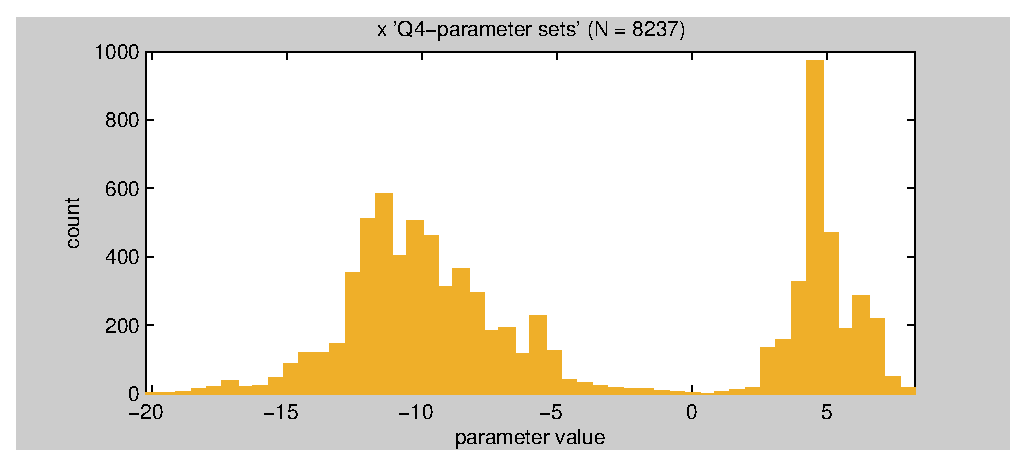
\includegraphics[width=\linewidth , keepaspectratio]{./../eps/mmsodaMargHist.eps}
  \caption{Histogram for the Q4 parameter sets for the double-normal model.}
  \label{fig:mmsodaMargHist}
\end{figure}


\smallq{Refer to the documentation on how to use \texttt{mmsodaPlotSeq}\index{MMSODA functions!mmsodaPlotSeq@\texttt{mmsodaPlotSeq}}. Create another figure on the right side of your screen, in which you visualize the record of sequences. Use the options to hide the samples that were rejected as part of the Metropolis scheme. You result should look like Fig.~\ref{fig:mmsodaPlotSeq}.}


\begin{figure}[htb]
  \centering
    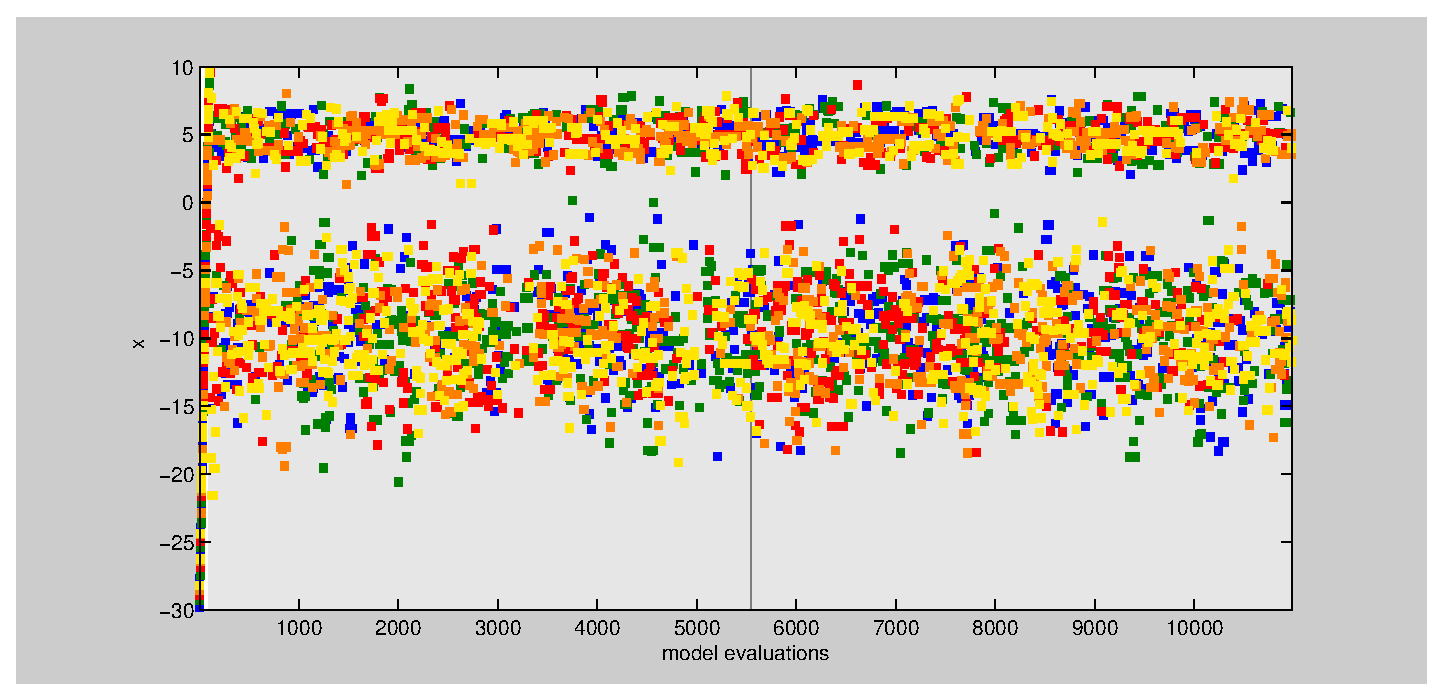
\includegraphics[width=\linewidth , keepaspectratio]{./../eps/mmsodaPlotSeq.eps}
  \caption{History of samples taken from the 1-D parameter space by \mbox{SCEM-UA} during optimization of the double-normal model.}
  \label{fig:mmsodaPlotSeq}
\end{figure}


%\smallq{Refer back to the documentation on the \texttt{mmsoda} function; specifically, browse through some of the configuration options for running MMSODA in `bypass' mode. Alter your `makeconf.m' with the options that you find useful, and re-run the optimization.}

\smallq{When you are satisfied with the way you set up MMSODA locally, you can make preparations for running it in parallel on the LISA cluster computer. Running on LISA requires a so-called `Makefile'\index{Makefile} as well as a jobscript\index{jobscript}, both of which are tricky to write yourself. Therefore, the MMSODA Toolbox for MATLAB comes with a function that helps you generate the correct files by asking a series of questions. At the MATLAB prompt, type:\\
\texttt{>> mmsodaPrepParallelFiles()}\index{MMSODA functions!mmsodaPrepParallelFiles@\texttt{mmsodaPrepParallelFiles}} \\
and use the following information to answer its questions:\\
\begin{enumerate}\label{li:answers-mmsodaPrepParallelFiles}
\item{the optimization will run on one of the login nodes;}
\item{we want not much verbal feedback from the program;}
\item{we don't want to use all the cores on the login node;}
\item{we want to start 4 processes;}
\item{we don't want to save the timing information.}
\end{enumerate}\\
(Note that \texttt{mmsodaPrepParallelFiles()} indicates the default answer with brackets, and that you can accept the default by simply pressing Enter.)
}

When \texttt{mmsodaPrepParallelFiles()} finishes, it prints a message in the command window that tells you what file it has just created. This file should be located in the current working directory. We will use it shortly to start the optimization on the cluster. You can take a look a its contents in Notepad or a similar program, but make sure not to change anything. Besides the jobscript, there should also be a new file called `Makefile'. Just like the jobscript, this is also a plain text file, so you can view its contents in Notepad as well. Again, make sure not to accidentally change anything.


\section{MMSODA in `bypass' mode; parallel execution}

\smallq{Use WinSCP or the alternative program of your choice to copy the `example1' and `mmsoda' directories, including all of their contents, to your storage on the cluster, i.e.\,anywhere under the `/home/$<$username$>$/' directory.}

When you are satisfied with the way you set up MMSODA locally, you can run it on the LISA cluster computer. In order to do so, we must first compile the software into a so-called `binary'\index{binary} or `executable'\index{executable}. You do not need to worry about how this works in detail, it is just a matter of running the Linux \texttt{make} command. \texttt{make} looks for a file called `Makefile' that was just created by \texttt{mmsodaPrepParallelFiles()}. Based on the contents of `Makefile', \texttt{make} collects all the relevant software (your model files, your objective functions, the MMSODA code, as well as the code that enables communication between the Master and the Workers) and creates two files that are necessary to run your code within MMSODA using multiple cores.

\subsection{Compiling MMSODA and your model code into a binary}

\smallq{Use PuTTY to start an SSH connection to the LISA cluster.}

\smallq{In the PuTTY terminal, load the MATLAB program and MPI programs by typing:\\
\texttt{module load matlab}\\
This command will not give any feedback on the success or otherwise of the command, but you could check by typing the following command:\\
\texttt{module list}\\
which should now include MATLAB. Next, type\\
\texttt{module load openmpi/gnu}\\
to load the MPI software.
}

\smallq{Use the \texttt{cd} command to set `example1' as your current directory if you hadn't already done so.}

\smallq{Now we are ready to compile. At the terminal, type:\index{Linux commands!make@\texttt{make}}\\
\texttt{make}\\
You should see some text scrolling over your screen---it takes about 60 seconds or so to complete. The \texttt{make} command looks for a file called `Makefile'\index{Makefile} in the current directory, and uses the information in it to correctly build the binary `matlabprog' and the library that it needs, called `libmmpi.so'.}

\smallq{After \texttt{make} finishes, list the directory contents with \texttt{ls -l} and verify that
you now have two extra files `matlabprog' and `libmmpi.so'.}

Starting the optimization requires that we adjust the `permission bits'\index{permission bits} for the `run-mmsoda.sh'\index{run-mmsoda.sh} file that was just created by \texttt{mmsodaPrepParallelFiles()}. Permission bits indicate what a specific user is allowed to do with a particular file. (You may know the same concept from Windows, where you can sometimes have `Read-only' versions of a file). The permission bits are listed as the first 10 columns in the output from \texttt{ls -l}:

\Needspace{12\baselineskip}

\begin{lstlisting}[style=basic,style=bash]
jspaaks@login1:~/esibayes/example1$ ls -l
total 204
drwxr-xr-x 2 jspaaks jspaaks     26 Jan 16 16:09 data
-rwxrwxr-x 1 jspaaks jspaaks 172792 Jan 18 11:57 libmmpi.so
-rw-r--r-- 1 jspaaks jspaaks    176 Jan 16 16:02 makeconf.m
-rw-r--r-- 1 jspaaks jspaaks    120 Jan 16 15:06 makeconstants.m
-rw-rw-r-- 1 jspaaks jspaaks   1357 Jan 16 16:10 Makefile
-rwxrwxr-x 1 jspaaks jspaaks  11969 Jan 18 11:57 matlabprog
drwxr-xr-x 2 jspaaks jspaaks     29 Jan 16 16:09 model
drwxr-xr-x 2 jspaaks jspaaks   4096 Jan 16 17:36 results
-rw-r--r-- 1 jspaaks jspaaks    580 Jan 18 13:26 run-mmsoda.sh
jspaaks@login1:~/esibayes/example1$
\end{lstlisting}

For `run-mmsoda.sh'\index{run-mmsoda.sh}, the permissions are set to \texttt{-rw-r--r--}. The first character \texttt{-} indicates that `run-mmsoda.sh' is a file (as opposed to a \texttt{d} which would indicate a directory). Characters 2, 3 and 4 (\texttt{rw-}) indicate what you, the currently logged-in user, is allowed to do with `run-mmsoda.sh'. Currently, you are allowed to read from (\texttt{r}) and write to (\texttt{w}) `run-mmsoda.sh'. The \texttt{-} character from the fourth column of \texttt{ls -l} indicates that you are currently not allowed to execute `run-mmsoda.sh' as a script.

\smallq{Change the permission bit for `run-mmsoda.sh' by typing at the prompt:\index{Linux commands!chmod@\texttt{chmod}}\\
\texttt{chmod u+x run-mmsoda.sh}\\
In normal English, this command translates to ``\texttt{Ch}ange the \texttt{mod}e of file `run-mmsoda.sh' by adding (\texttt{+}) the executable permission (\texttt{x}) for the current user (\texttt{u})''. Check that the permissions have changed to \texttt{-rwxr--r--}.}

\smallq{Now we are ready to start the optimization in parallel on the login node. At the beginning of the optimization, you will see a lot of text scrolling over your terminal screen which at this stage probably does not make much sense. Don't worry if you don't understand it---we will look at it in greater detail later. Eventually, you'll get messages along the lines of `Evaluating parameter sets 1-100', `Evaluating parameter sets 101-120', etc. Start the optimization by typing at the terminal:\\
\texttt{./run-mmsoda.sh}\\
(Don't omit the \texttt{./} at the beginning, otherwise it won't work.)
}

%\smallq{\textit{Parallel execution is actually slower than in series due to Amdahl's Law and due to the presence of other users on the login nodes.}\index{todo}}

\smallq{After the optimization finishes, the results need to be transferred to your local system. Copy the contents of `example1/results/' from the remote system to `example1/results/' on your local machine (you can overwrite the old files in `example1/results/' on your local machine if you want).
}

\smallq{On your local machine, clear the workspace, and load MMSODA's output variables using:\\
\texttt{ >> load(\squote{./results/bypass-so-results.mat})}\\
You can now use any of the MMSODA visualizations (or MATLAB visualizations for that matter), in just the same way as if the results had been calculated locally.}


\smallq{Now that you know what information goes where for MMSODA in `bypass' mode, it may be useful to review some of the other examples in the `esibayes' directory. On your local machine, explore the configurations for a few of the other `bypass' mode directories. Try running MMSODA for those configurations, but make sure MATLAB is set to the correct working directory when \texttt{mmsoda} is started.}


% % % % % % % % % % % % % % % % % % % % % % % % % % % % % % % % % %

\section{MMSODA in `scemua' mode; sequential execution}

Now that we have a working example of MMSODA in `bypass' mode, let's try our hand at something a little more difficult: optimizing the parameters of a dynamic model\index{MMSODA!scemua mode}. This works in more or less the same way as the bypass mode, except that the likelihood is determined by comparing a model prediction to observations, while taking into account the uncertainty of the latter. Let's first make a small digression and look at the general structure of dynamic models. Such models simulate the behavior of a number of states over time. As an example, Fig.~\ref{fig:states-and-flows} shows a system in which there are two states. The first state is the water level in a tank which has a small hole in the bottom. The second state is the water level in a tank that has no leaks. The first tank discharges into the second. The rate of discharge $Q$ is dependent on the volume of water in the tank $V_{tank_1}$ and on a resistance parameter $R$ (if there is a big leak in the first tank, the resistance is low, but if the leak is only small, the resistance is high). The model simulates discharge as follows:
\begin{equation}\label{eq:flow-from-tank1}
Q = \frac{V_{tank_1}}{-R}
\end{equation}

Given the state of the upper tank at a given point in time $V_{tank_1}(t)$, Eq.\,\ref{eq:flow-from-tank1} may be used to calculate the corresponding flow at time $t$. Furthermore, the current state $V_{tank_1}(t)$ and flow $Q(t)$ may be used to simulate the state at a later time, $t+\Delta{}t_{sim}$, provided that $\Delta{}t_{sim}$ is sufficiently small:
\begin{equation}\label{eq:numerical-integration-tank1}
V_{tank_1}(t+\Delta{}t_{sim}) = V_{tank_1}(t) + Q(t)*\Delta{}t_{sim}
\end{equation}
\begin{equation}\label{eq:numerical-integration-tank2}
V_{tank_2}(t+\Delta{}t_{sim}) = V_{tank_2}(t) - Q(t)*\Delta{}t_{sim}
\end{equation}

If the initial state of the system $V_{tank_1}(t_0)$ and $V_{tank_2}(t_0)$ is known, and if the resistance parameter $R$ has been assigned, repeated application of Eqs.\,\ref{eq:flow-from-tank1}--\ref{eq:numerical-integration-tank2} thus enables constructing a time series of simulated values for $V_{tank_1}$ and $V_{tank_2}$.

\begin{figure}[htb]
  \centering
    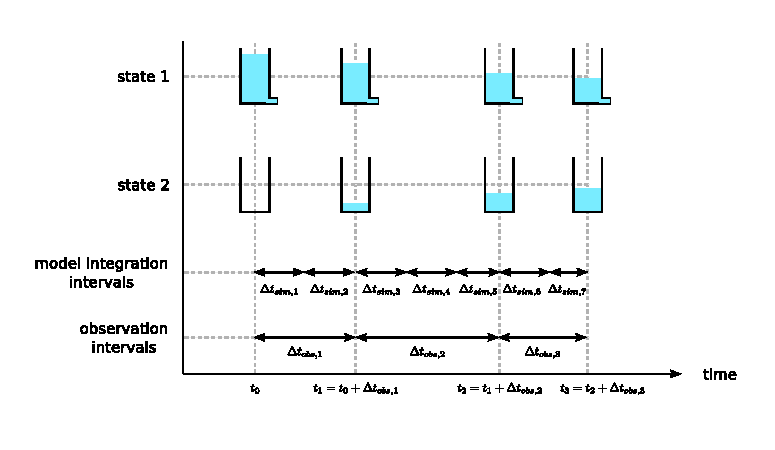
\includegraphics[width=\linewidth,keepaspectratio]{./../eps/states-and-flows.eps}
  \caption{The general structure of dynamic models.}
  \label{fig:states-and-flows}
\end{figure}

It is quite common that not all the parameter values are known beforehand, so in order to make predictions with the model, it becomes necessary to estimate the model parameter values by comparing simulation results to observations of the system's states. The model must therefore be set up such that it returns the system's state at the times for which an observation is available, otherwise the comparison isn't much use. Since the time interval between observations $\Delta{}t_{obs}$ can be (much) larger than the model integration interval $\Delta{}t_{sim}$, multiple model integration steps are often needed in between observation times. Listing~\ref{list:lintank-script} shows a simple MATLAB script that implements the system depicted in Figure~\ref{fig:states-and-flows}.  A copy of the script has been included as `other/lintank\_script.m'.

\Needspace{7\baselineskip}

Over the next few exercises, we will:
\begin{enumerate}
\item{prepare a `constants.mat',}
\item{prepare a `conf.mat',}
\item{prepare the main model m-file by adapting `lintank\_script.m' such that it can be used within the MMSODA framework,}
\item{construct a likelihood function.}
\end{enumerate}
%The above four steps are necessary for all types of optimization except `bypass'.


\smallq{Before we start, make sure you understand how the `lintank\_script.m' works by studying Listing~\ref{list:lintank-script} and running through it line-by-line using MATLAB's debugging capabilities.}

\Needspace{64\baselineskip}
\lstinputlisting[style=basic,style=matlab,style=numbered,style=spacious,caption={Simple MATLAB script that implements the system depicted in Figure~\ref{fig:states-and-flows}. A copy of this script has been included as `other/lintank\_script.m'.},label=list:lintank-script]{./../m/lintank_script.m}

\begin{figure}[htb]
  \centering
    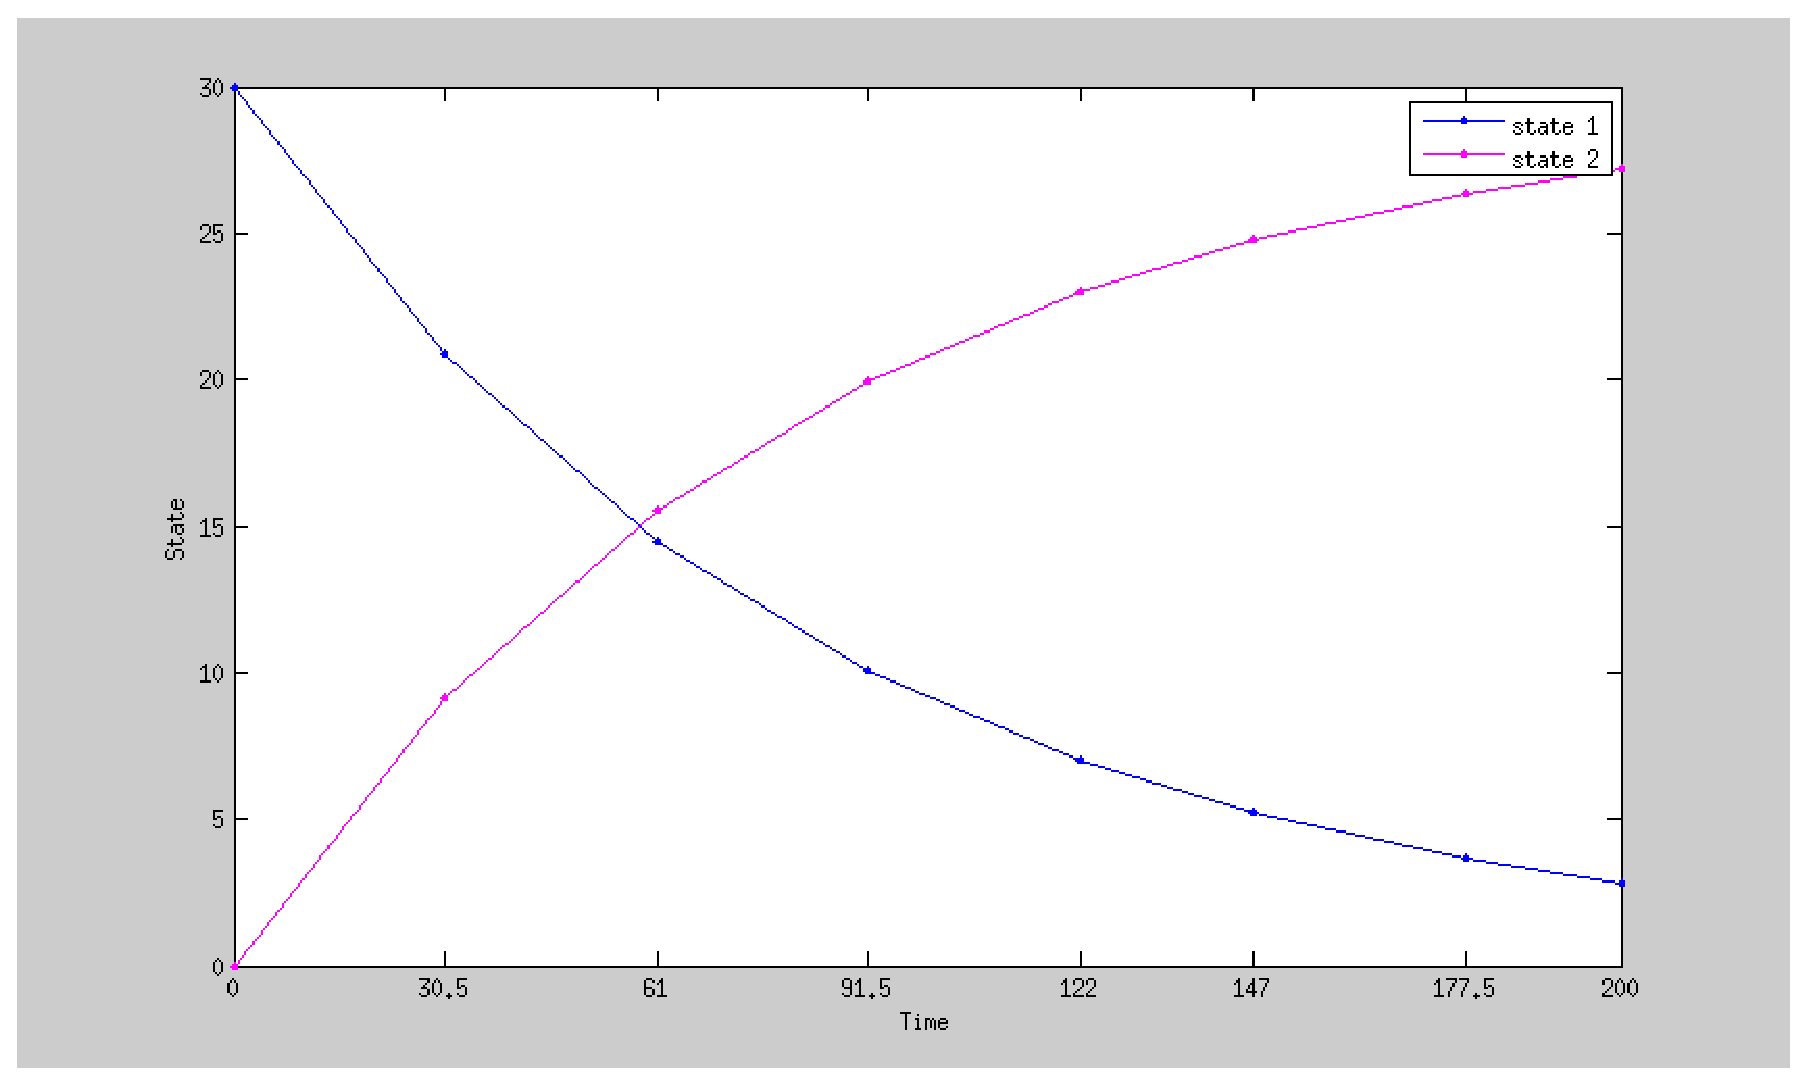
\includegraphics[width=\linewidth,keepaspectratio]{./../eps/result-of-lintank-script.eps}
  \caption{Result of running the code from Listing~\ref{list:lintank-script}.}
  \label{fig:result-of-lintank-script}
\end{figure}


\smallq{Create a new directory structure with the required subdirectories just like you did before. Call the top directory `example2'. Verify that the `example2' directory is at the same level as the `mmsoda-toolbox' directory.}

\smallq{Read the MMSODA documentation on `the dynamic model' (see Figure~\ref{fig:doc-the-dynamic-model}).}

\begin{figure}[htb]
  \centering
    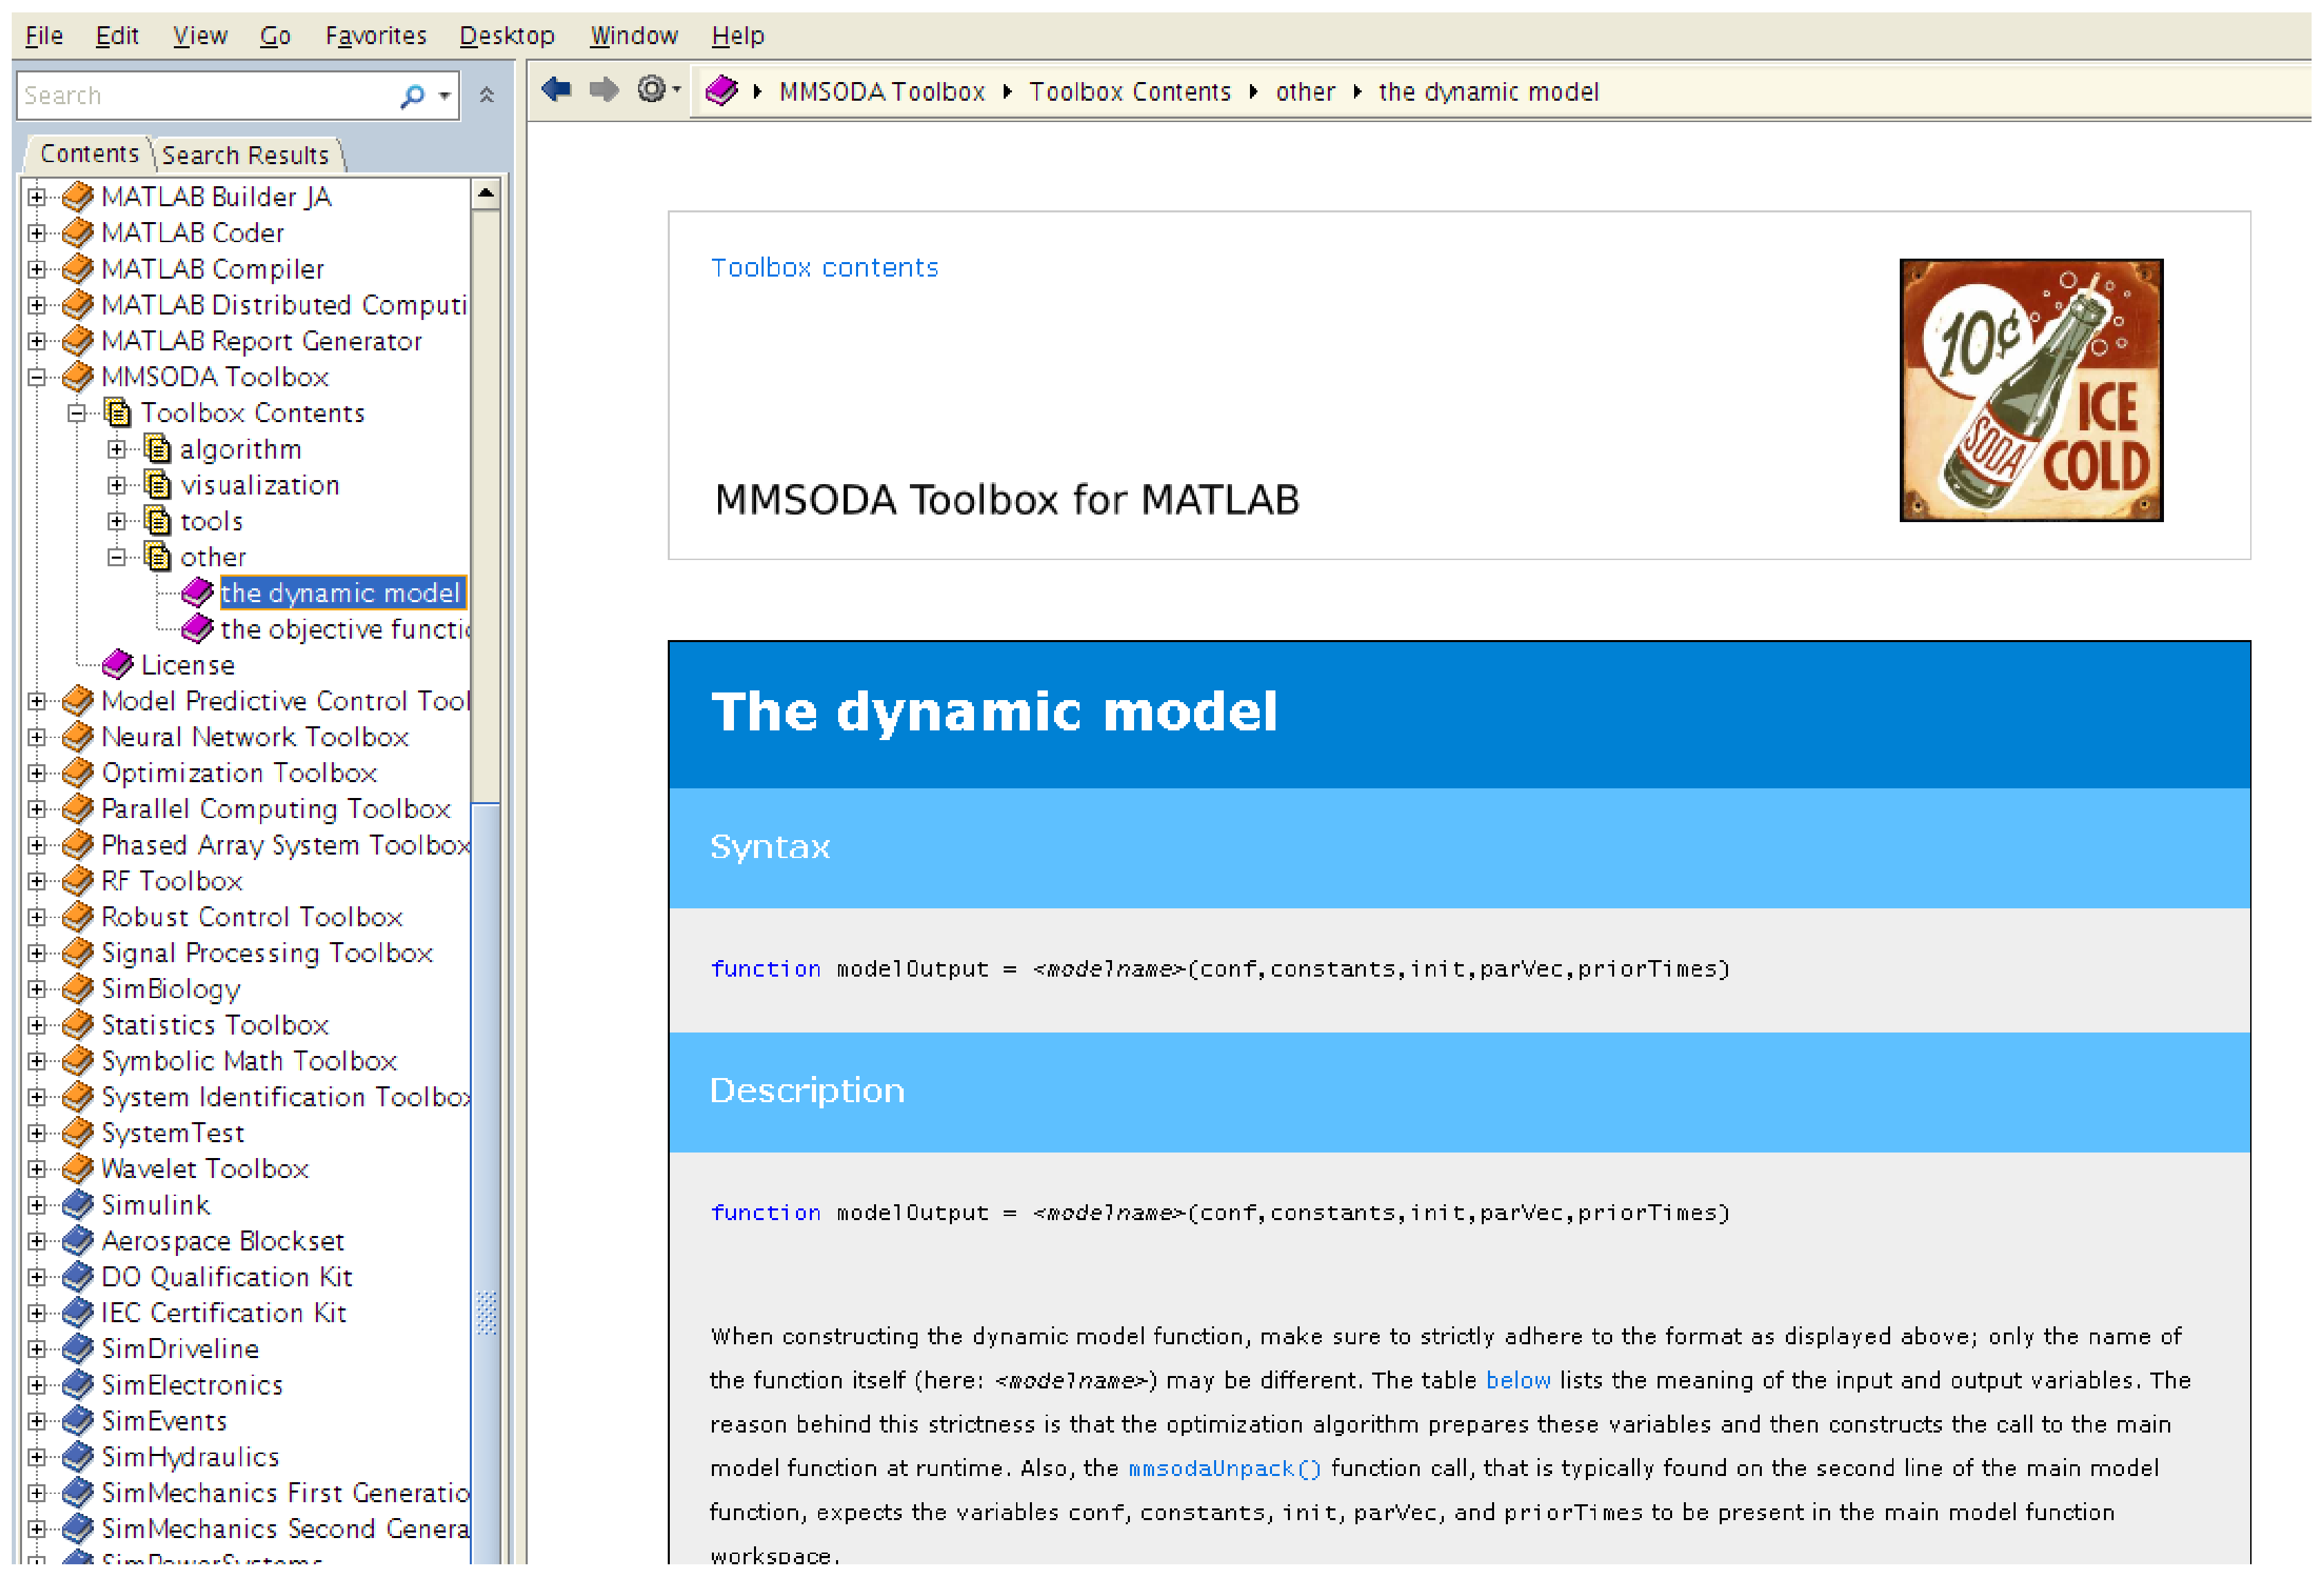
\includegraphics[width=\linewidth,keepaspectratio]{./../eps/doc-the-dynamic-model.eps}
  \caption{MATLAB documentation on how to set up the dynamic model.}
  \label{fig:doc-the-dynamic-model}
\end{figure}

In the initialization part of Listing~\ref{list:lintank-script}, 10 variables (\texttt{R}, \texttt{state1Init}, \texttt{state2Init}, \texttt{priorTimes}, \texttt{tNow}, \texttt{tEnd}, \texttt{dtSimDefault}, \texttt{rec}, \texttt{state1}, and \texttt{state2}) are created, but only some of these need to be included in `constants.mat'. For example, \texttt{R} does not need to be in `constants.mat' because its value will be determined by MMSODA: the variable \texttt{R} is assigned by \texttt{mmsodaUnpack} (which uses the input argument \texttt{parVec} to do so). Similarly, \texttt{priorTimes} and its derivatives \texttt{tNow} and \texttt{tEnd} do not need to be in `constants.mat' because \texttt{priorTimes} is an input argument, too. \texttt{state1}, \texttt{state2}, and \texttt{rec} are all derived from other variables, so they do not need to be part of `constants.mat' either. Essentially, all we need is \texttt{state1Init}, \texttt{state2Init}, and \texttt{dtSimDefault}.

\smallq{Write `makeconstants.m'.}

\smallq{Create a new m-file called `makeconf.m' just like you did before, but this time make sure that the m-file lists the necessary configuration variables for a `scemua' optimization. Refer to the configuration variables table in the MATLAB documentation of \texttt{mmsoda}, and use the information below to set up the optimization:
\begin{enumerate}
\item{Set \texttt{modeStr} to \texttt{\squote{scemua}};}
\item{Set \texttt{modelName} to \texttt{\squote{lintank}}. (We will create `lintank.m' later);}
\item{Set \texttt{objCallStr} to \texttt{\squote{calcLikelihoodState}}. (We will create `calcLikelihoodState.m' later);}
\item{Set \texttt{parNames} to a cell array of strings with the name of the resistance parameter exactly as used in the dynamic part of the model: \texttt{\{\squote{R}\}}. \texttt{R} is the only parameter that will be optimized; }
\item{For the upper boundary of the parameter space, use 1000.0;}
\item{For the lower boundary of the parameter space, use 80.0;}
\item{Fill in the \texttt{priorTimes} values by copying from `lintank\_script.m';}
\item{Set \texttt{nOutputs} to 2.}

\end{enumerate}
} % smallq


\smallq{Copy `lintank\_script.m' to your `model' subdirectory. Rename it to `lintank.m'.}

\smallq{Adapt `lintank.m' to be a function. Refer to the MMSODA documentation on the dynamic model for the proper way of constructing the function's input and output arguments. Remove all lines from the initialization part that are obsolete given that we want to run it within the MMSODA framework. Afterwards, your code should look like that of Listing~\ref{list:lintank-function-1-19}.}

\needspace{20\baselineskip}
\lstinputlisting[style=basic,style=matlab,style=numbered,style=spacious,caption={First 19 lines of `lintank.m'. You can find a copy of this script at `other/lintank.m'.},label=list:lintank-function-1-19,firstline=1,lastline=19]{./../m/lintank.m}


Next, we need to make sure that the function returns the correct values---we want it to return an array of size \texttt{nOutputs x nPrior}. The $n^{th}$ column in the output argument \texttt{modelOutput} must contain the values pertaining to the $n^{th}$ time in \texttt{priorTimes}. Listing~\ref{list:lintank-function-61-70} shows a simple way of accomplishing this.

\lstinputlisting[style=basic,style=matlab,style=numbered,style=spacious,caption={Last 10 lines of `lintank.m'. You can find a copy of this script at `other/lintank.m'.},label=list:lintank-function-61-70,firstline=61,lastline=70,firstnumber=61]{./../m/lintank.m}



\smallq{Now it's time to test if everything works so far. Make sure MATLAB is in the correct working directory (i.e.\,one level higher than your `data', `model', and `results' directories). At the MATLAB prompt type:\\
\texttt{>> [evalResults,critGelRub,sequences,metropolisRejects,conf] = mmsoda()}\\
and press Enter. If all goes well, MMSODA will start printing various messages to your screen. You should see the message `\texttt{Evaluating parameter sets 1-100}', and if you haven't commented out the visualization part in `lintank.m', you should see 100 plots being made before MMSODA crashes with the following error:}
\begin{lstlisting}[style=basic,style=bash]
Error using eval
Undefined function 'calcLikelihoodState' for input arguments of type 'struct'.
>>
\end{lstlisting}
The error is because MMSODA refers to the configuration variable \texttt{objCallStr}, which you set to \texttt{\squote{calcLikelihoodState}} earlier on. When MMSODA attempts to run \texttt{calcLikelihoodState}, this results in an error because we still have to create `calcLikelihoodState.m'.

\smallq{Read the documentation about the objective function (see Figure~\ref{fig:doc-the-objective-function}).}

\begin{figure}[htb]
  \centering
    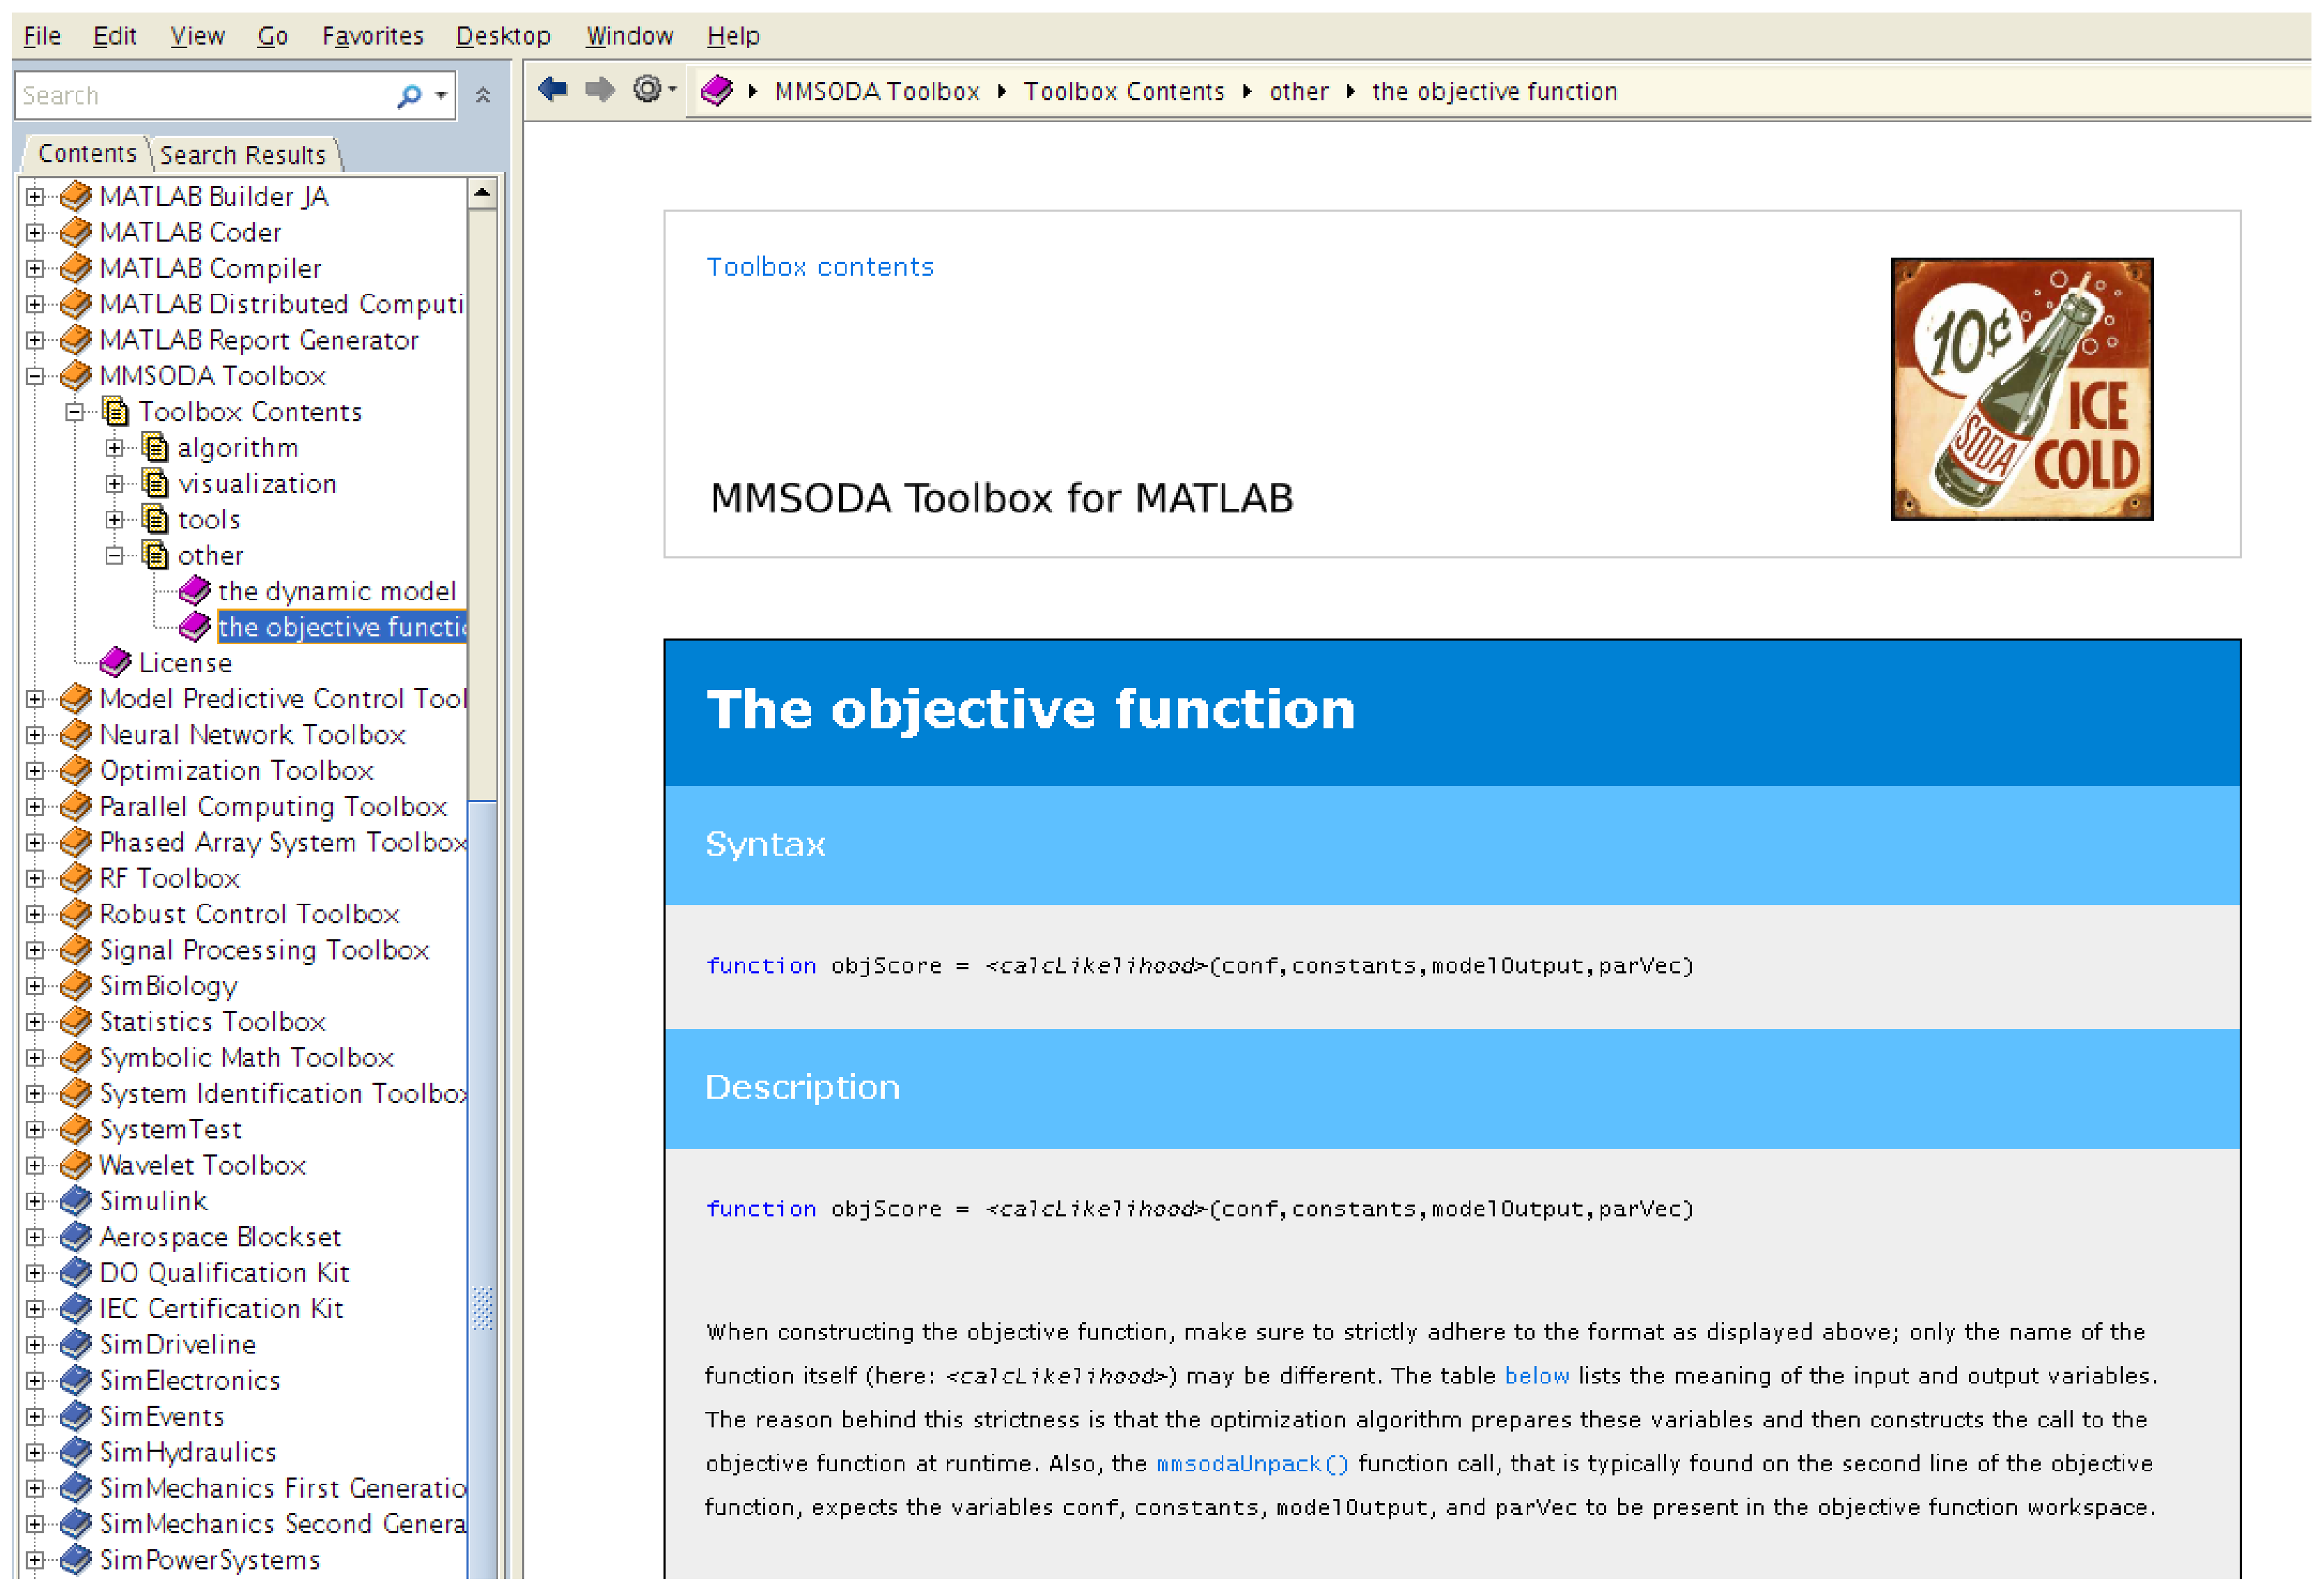
\includegraphics[width=\linewidth,keepaspectratio]{./../eps/doc-the-objective-function.eps}
  \caption{MATLAB documentation on how to set up the objective function.}
  \label{fig:doc-the-objective-function}
\end{figure}

\smallq{Create a new m-file in the `./model' subdirectory, and call this file `calcLikelihoodState.m'. Refer to the documentation and make sure the first line of the objective function is correct.}

The objective function we will use is related to the sum of squared residuals \index{sum of squared residuals} or SSR\index{SSR}:
\begin{equation}\label{eq:SSR}
\mathrm{SSR} = \displaystyle\sum\limits_{t=1}^{n_o}(\hat{x}_{t}-\tilde{x}_{t})^2
\end{equation}
with $\hat{x}_{t}$ the $t^{\mathrm{th}}$ predicted value of $x$, $\tilde{x}_{t}$ the $t^{\mathrm{th}}$ observed value of $x$, and $n_o$ the total number of observations. Note that the number of observations $n_o$ is one less than the number of elements in \texttt{conf.nPrior}, since the first column in \texttt{modelOutput} is not calculated by the model, but instead contains the initial values of the model output variables.

However, we can't use the SSR directly as an objective score, because the SSR is not a log-likelihood (or a probability, for that matter). This problem is easily resolved though, by using the following objective function\footnote{Skip forward to Appendix~\ref{ch:likelihoods-in-optimization} to see how this was derived.}:
\begin{equation}\label{eq:objScore}
\ell = -\frac{1}{2} \cdot{} n_o \cdot{} \mathrm{ln}\left(\mathrm{SSR}\right)
\end{equation}

In order to calculate the SSR, we need some observations. These have been prepared already and are located in the `other' directory.

\smallq{Copy `other/lintank-obs.mat' to your `./data' directory.}

\smallq{In `calcLikelihoodState.m', add \\
\texttt{load({\squote{./data/lintank-obs.mat}},\squote{obs},\squote{obsTimes})}
}% smallq


Now that we have the observations in the workspace, we still need to select the corresponding simulations from the \texttt{modelOutput} variable. Refer to the documentation on the objective function for a description. We want to select all values pertaining to the first state (since this is the state that we have observations for). We can do so by:

\needspace{5\baselineskip}

\begin{lstlisting}[style=basic,style=matlab]
% row of interest in 'modelOutput' is #1
r = 1;
nPriors = size(modelOutput,2);
nObs = nPriors-1;

% extract the relevant row from 'modelOutput'
sim = modelOutput(r,1:nPriors);

% Calculate the SSR, but ignore the first entry in 'obs' and 'sim' because those are always
% exactly the same anyway
ssr = sum((obs(1,2:nPriors)-sim(1,2:nPriors)).^2);

% use the SSR to calculate the likelihood
objScore = -(1/2) * nObs * log(ssr);
\end{lstlisting}

\smallq{Add the command lines above to your \texttt{calcLikelihoodState} in order to let it calculate the SSR and the objective score according to Eq.~\ref{eq:objScore}.}

\smallq{Make sure you are still in the right working directory. At the MATLAB prompt, type:\\
\texttt{>> [evalResults,critGelRub,sequences,metropolisRejects,conf] = mmsoda()}\\
}


Currently, \texttt{calcLikelihoodState} loads the observations from file every time it needs to calculate the \texttt{objScore}. Since file operations are much slower than memory operations, it is more efficient to load the observations just once (during creation of the constants), and then keep them in the computer's memory.

\smallq{Cut the \texttt{load} statement from \texttt{calcLikelihoodState} and paste it into `makeconstants.m'. Make sure to re-run \texttt{makeconstants()}, otherwise `./data/constants.mat' will remain unchanged.}

\smallq{Re-read the documentation on MMSODA's \texttt{mmsodaUnpack()} function. Go back to `calcLikelihoodState.m' and use \texttt{mmsodaUnpack()} to make the observations available in the objective function's workspace. Restart the optimization to check if everything works.}


%\smallq{\textit{some interpretation of results}.\index{todo}}

\section{MMSODA in `scemua' mode; parallel execution}

\smallq{Generate a `Makefile' and a jobscript using \texttt{mmsodaPrepParallelFiles()}. Use the same answers as those given on page~\pageref{li:answers-mmsodaPrepParallelFiles}. }

\smallq{Copy the working directory to LISA using WinSCP or an alternative program. Make sure the directory is at the same level as the `mmsoda-toolbox' directory that should still be present on the remote system.}

\smallq{Use PuTTY to start an SSH connection to the LISA cluster.}

\smallq{Load the necessary software modules and compile your m-files together with the MMSODA m-files.}

\smallq{Add the executable permission to `run-mmsoda.sh'.}

\smallq{Start the optimization on the login node.}

So far, we've run our optimizations on one of the login nodes. These nodes are intended for testing small problems and for development work. However, if you want to do some real calculations, then it becomes necessary to submit your job to the PBS queue (as discussed in Chapter~\ref{ch:getting-started}).

\smallq{Submitting your optimization to the PBS scheduler requires a slightly different jobscript. On your local system, run \texttt{mmsodaPrepParallelFiles}, but this time indicate that you want to run your optimization as a PBS jobscript, without much verbal feedback, and that you want 00:15:00 walltime on 1 node. We are not interested in saving the timings for the moment. When \texttt{mmsodaPrepParallelFiles} finishes, it prints the name of the file it just created (`jobscript-mmsoda.pbs') to the command window. Copy this file to the working directory on the remote system.}


\smallq{Make sure that PuTTY is in the right directory and type:\\
\texttt{qsub jobscript-mmsoda.pbs}\\
to add the optimization to the scheduler's queue. Note that it is not necessary to change the permission bits for `jobscript-mmsoda.pbs' when it is simply an input argument to \texttt{qsub}, rather than a program in its own right. Furthermore, it is also not necessary to re-compile your program, since we did not change anything in the code---we're just submitting to a different queue.}

\smallq{Use the tools discussed in Chapter~\ref{ch:getting-started} (e.g.\,\texttt{qstat}, \texttt{showq}, \texttt{showstart}, \texttt{checkjob}) to check on the status of your job.}

%\smallq{When the job has finished, copy the contents of the `./results' subdirectory to your local system for further analysis.}

\subsection{Standard output and standard error}

This is probably as good a time as any to look in more detail at some of the outputs that MMSODA generates. On the remote machine, there should now be a file `./results/jobscript-mmsoda.pbs.\textbf{o}XXXXXXX' (those X's represent the job id number). This file contains the standard \textbf{o}utput of our parallel optimization program. Whenever any of the parallel processes would normally print some message to the command window, on LISA that text will instead end up in the standard output file\index{standard output file}. The standard output file (and its sister, the standard \textbf{e}rror file\index{standard error file} `./results/jobscript-mmsoda.pbs.\textbf{e}XXXXXXX') is interesting because it is the first place to look if something is not going like it should.

It is not necessary for you to fully understand what all lines in the standard output mean, but having just a general idea can save you a lot of time and frustration when you run into trouble. Most often, tracking an error is just a matter of spotting the difference between the output that you see when everything is working and when it's not. If nothing else, you can send the standard output file to one of the LISA administrators, such that (s)he may assist you better in solving your problem.

The standard output files that are generated during MMSODA optimizations typically consist of three parts: first, there is the output that was written when everything was being set up for the MMSODA run; second, there is a middle part that contains output that would be displayed in MATLAB's command window if you were running MMSODA on your local machine. Finally, the third part contains some text that the LISA system adds to every job's standard output. Listings~\ref{li:standard-out-first-part} and \ref{li:standard-out-last-part} show the most interesting parts of the standard output for a single-objective MMSODA optimization in `scemua' mode. Much of the lines in the first part are generated by bash commands\footnote{See page~\pageref{word:bash} in Chapter~\ref{ch:getting-started}.} from the jobscript. For example, it includes the ID of the job (lines 3--4), an \texttt{ls -l} overview of the files in the current directory (lines 12--22), an overview of the type of CPU in each node (lines 29--45), an overview of the nodes which have been assigned to this job by the scheduler (lines 47--63; the name of each node occurs as many times as there are CPUs in it, so in this case there are 16 `r41n3' entries). Then the necessary modules are loaded and an overview is printed of the available modules (lines 65--77). Next, lines 79--81 add the current directory to the environment variable LD\_LIBRARY\_PATH to make sure that `libmmpi.so' can be located by the compiled MATLAB program. The next few lines (83--85) prepare a temporary directory that is needed by the compiled MATLAB program. Lines 87--117 print results of the Linux \texttt{ldd}\index{Linux commands!ldd@\texttt{ldd}} command. \texttt{ldd} prints the location of the libraries that are needed by our compiled MATLAB program (`matlabprog') and by the library that we made (`libmmpi.so'). After every \texttt{=>} sign in the \texttt{ldd} result, there should be an entry; if it says `not found', something is wrong. For example, if we would not have added the current directory to the LD\_LIBRARY\_PATH, line 91 would say `\texttt{libmmpi.so => not found}'. Next, lines 119--176 constitute a list of so-called `symbols' that are present inside the `mmsoda-toolbox/comms/helper.o' file. This file is a C-language object file needed for MPI communication between nodes in the cluster. The next few lines (178--195) show that the MATLAB engine was indeed started 16 times (once for every CPU in the node), and each of those 16 instances of MATLAB recognized immediately that there was no display (since the nodes inside a cluster are primarily set up for calculation, and are therefore not connected to a screen).


The middle part of the standard output is what you normally see in the command window; it starts with a disclaimer message that is generated by the MMSODA code (lines 197--198). Most of the remainder of the middle part consists of `Evaluating parameter sets X-Y' messages (lines 203--902), indicating the progress of the MMSODA algorithm.

The last part of the standard output file (lines 906--920) is always added by the LISA system. It provides an overview of the resources that were used in executing the job.

\Needspace{15\baselineskip}

\lstinputlisting[style=basic,style=bash,style=numbered,style=spacious,breaklines=true,breakindent=0,breakautoindent=false,prebreak=\mbox{{\color{blue}\hspace*{1em}$\swarrow$}},postbreak=\mbox{{\color{blue}$\rightarrow$\hspace*{1em}}},caption={First part of the standard output file. Lines that were too long to fit on the page were wrapped; this is indicated with the line break \mbox{{\color{blue}$\swarrow$}} and line continuation \mbox{{\color{blue}$\rightarrow$}} symbols.},label=li:standard-out-first-part,firstline=1,lastline=207]{./../res/jobscript-mmsoda.pbs.o6734963}

\Needspace{15\baselineskip}

\lstinputlisting[style=basic,style=bash,style=numbered,style=spacious,breaklines=true,breakindent=0,breakautoindent=false,prebreak=\mbox{{\color{blue}\hspace*{1em}$\swarrow$}},postbreak=\mbox{{\color{blue}$\rightarrow$\hspace*{1em}}},caption={Last part of the standard output file. Lines that were too long to fit on the page were wrapped; this is indicated with the line break \mbox{{\color{blue}$\swarrow$}} and line continuation \mbox{{\color{blue}$\rightarrow$}} symbols.},label=li:standard-out-last-part,firstline=898,lastline=920,firstnumber=898]{./../res/jobscript-mmsoda.pbs.o6734963}



\subsection{Analyzing the parallelization overhead}

When dealing with parallel programs, it is often useful to monitor how much time is lost in parallelization overhead in relation to the CPU time (recall Fig.~\ref{fig:walltime-comparison}). The MMSODA Toolbox for MATLAB enables you to record and visualize the timings of all relevant events (sending and receiving data, serializing\index{serializing}\footnote{Serialization is the process of collecting all the arrays that need to be sent over to a different machine, such that the arrays occupy a consecutive part of the computer's memory. This part of the memory can then be sent to another machine.} and deserializing\index{deserializing}, waiting for input, etc.) on all nodes that have been assigned to the job. Recording the timings does slow the optimization down slightly, so the default behavior is not to record any events. However, enabling the time-keeping functionality is simply a matter of re-running the \texttt{mmsodaPrepParallelFiles()} function, and answering `a : yes' to the last question `Would you like to save the timings?'.

\smallq{Re-run \texttt{mmsodaPrepParallelFiles()} and enable time-keeping. Copy the newly created jobscript to the cluster. Submit the new jobscript using \texttt{qsub}.}

\smallq{After the job finishes, copy the contents of the `./results' directory from the remote system to your local system.}


\smallq{Read the documentation on \texttt{mmsodaAnalyzeTimings}\index{MMSODA functions!mmsodaAnalyzeTimings@\texttt{mmsodaAnalyzeTimings}} and visualize the timings for the linear tank example. Would you say that parallel optimization of the linear tank model is a coarse-grained or a fine-grained problem?}

At this point, you are familiar with MMSODA in `bypass' mode and in `scemua' mode, and you know how to run MMSODA optimizations locally as well as on the LISA cluster. In the next few sections, we will cover the `reset' mode and `soda' modes, but the important point is that the workflow as you know it from the previous projects (as summarized in Fig.~\ref{fig:mmsoda-workflow}) is the same for all MMSODA projects.

\begin{figure}[htbp]
  \centering
    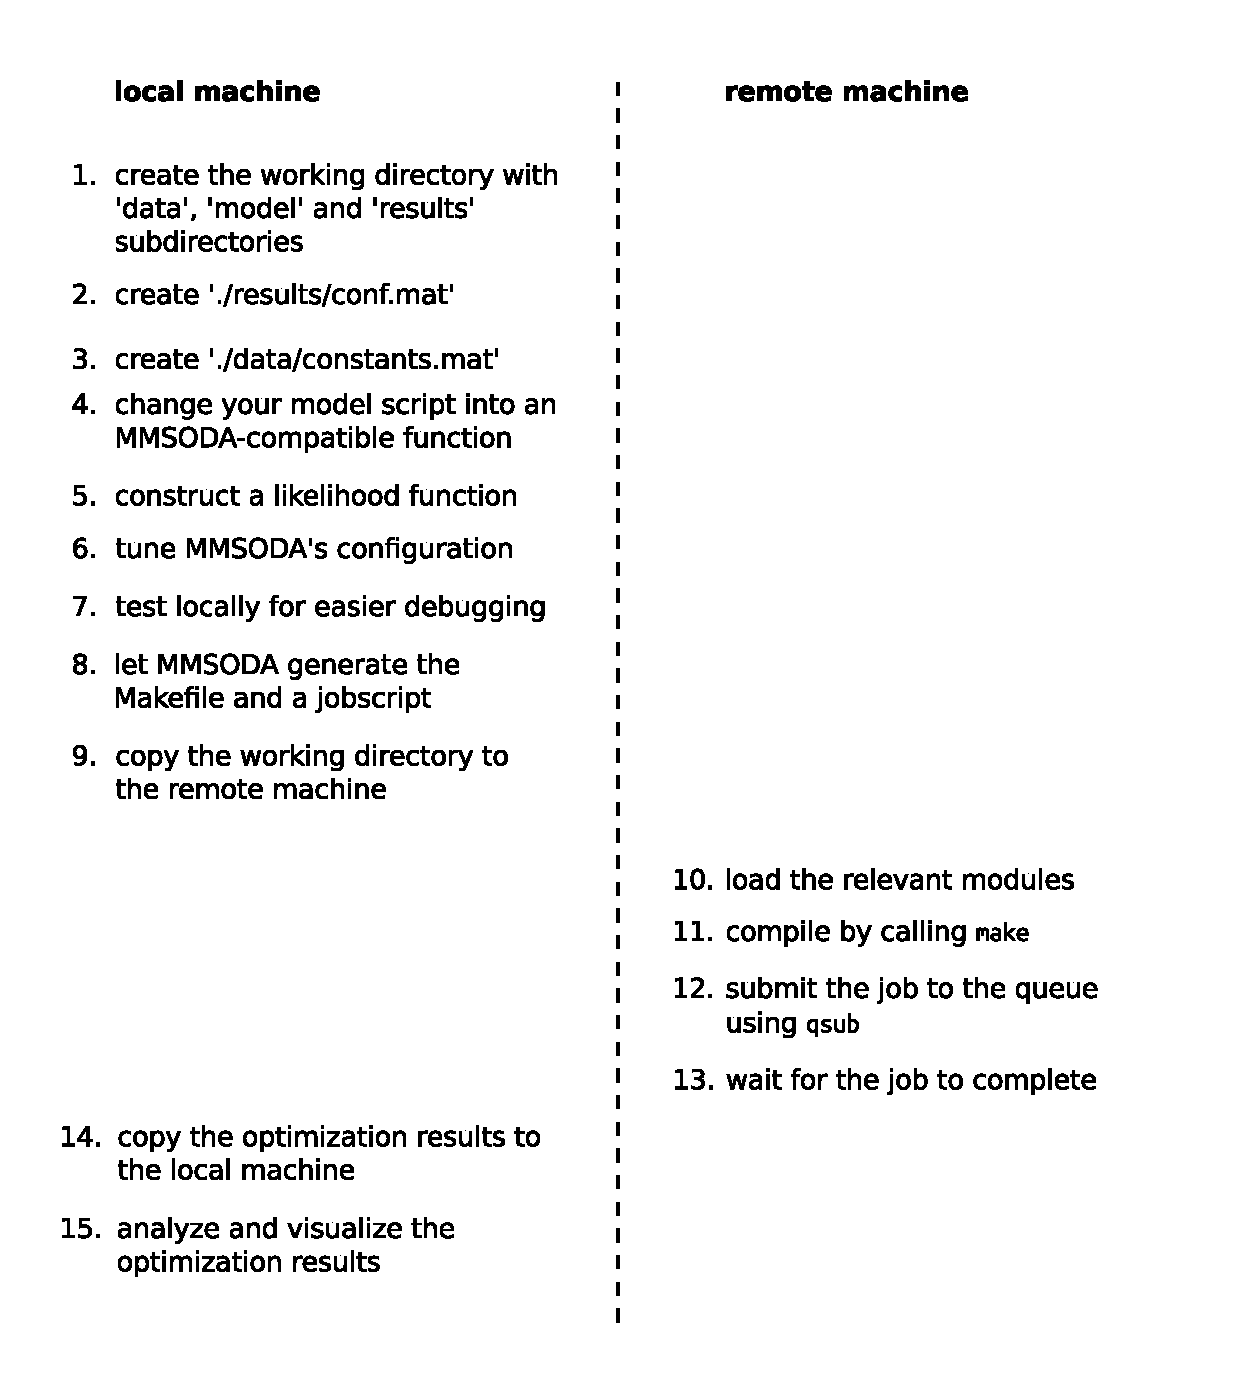
\includegraphics[width=0.85\linewidth,keepaspectratio]{./../eps/mmsoda-workflow.eps}
  \caption{Typical workflow for setting up MMSODA optimizations. Note that the items under `remote machine' are executed in a terminal program such as PuTTY.}
  \label{fig:mmsoda-workflow}
\end{figure}


\smallq{Now that you know what information goes where for MMSODA in `scemua' mode, it may be useful to review some of the other examples in the `esibayes' directory. On your local machine, explore the configurations for a few of the other `scemua' mode directories. Run MMSODA for those configurations, but make sure MATLAB is set to the correct working directory when \texttt{mmsoda} is started.}


\section{MMSODA in `reset' mode; sequential execution}

\smallq{On your local system, make a copy of the `example2' directory, and rename the copy to `example3'. Clean up the `example3' directory by removing `matlabprog', `libmmpi.so', `Makefile', `jobscript-mmsoda.pbs' as well as any results pertaining to the `example2' case. Set your MATLAB working directory to the newly created `example3' directory.}

\smallq{Remove the `constants.mat' and `lintank-obs.mat' files from the `example3/data' directory. Copy `lintank-obs-unobserved-input.mat' from the `other' directory to `example3/data'.}

\smallq{On the MATLAB command line, load the \texttt{obsTimes} and \texttt{obs} variables from the `./data/lintank-obs-unobserved-input.mat' file by typing:\\
\texttt{ >> load(\squote{./data/lintank-obs-unobserved-input.mat},\squote{obsTimes},\squote{obs})}}

\smallq{Visualize the data that were just loaded by:\\
\texttt{ >> plot(obsTimes,obs(1,:),\squote{-b.})}\\
Your figure should be similar to Fig.~\ref{fig:lintank-obs-unobserved-input}.}

\begin{figure}[htb]
  \centering
    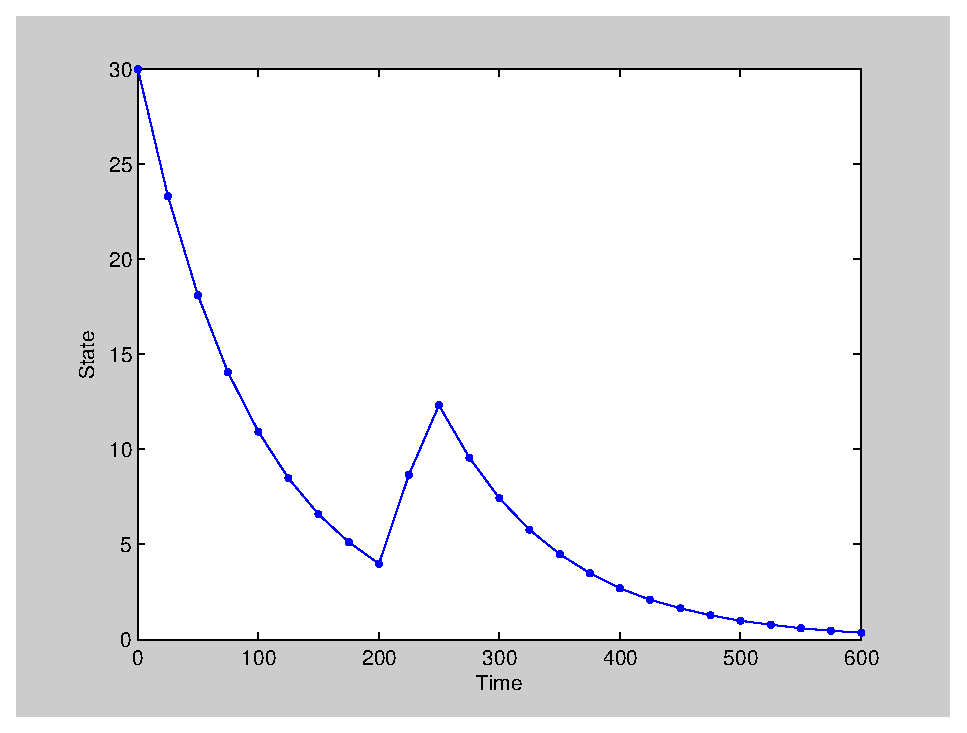
\includegraphics[width=\linewidth,keepaspectratio]{./../eps/lintank-obs-unobserved-input.eps}
  \caption{Simple \texttt{plot} of the data in `./data/lintank-obs-unobserved-input.mat'. The true value of the resistance parameter in this figure is 100.}
  \label{fig:lintank-obs-unobserved-input}
\end{figure}

From Fig.~\ref{fig:lintank-obs-unobserved-input}, it is clear that something happened around Time=200--250. It seems that water was added to the upper tank---that is to say, the upper tank has been subjected to an unobserved input. This kind of error is very common in hydrology; for example if the linear tank simulates the streamflow from a particular catchment, it can sometimes happen that streamflow in the river increases (as in Fig.~\ref{fig:lintank-obs-unobserved-input}), without any rain being recorded during the preceding days. Most often, these kinds of apparent impossibilities are explained by a rainstorm which did indeed pass over (some of) the catchment, but which missed the location of the rain gauge. Observational error like that can play havoc with the effectiveness of the calibration, as we shall see shortly.

In this section, we will look at what happens if we take a naive approach to calibrating the lintank model to the data of Fig.~\ref{fig:lintank-obs-unobserved-input}. For this, we need to make a few changes in the MMSODA configuration. For example, we need the model to generate predictions at \texttt{priorTimes = [0:25:600]}, and we want to use the data from `./data/lintank-obs-unobserved-input.mat' in the objective function.

\smallq{Make the necessary changes to `makeconf.m' and `makeconstants.m' to implement these changes. Also change the value of the \texttt{dtSimDefault} model constant to 2.0 and set the lower and upper boundaries of the parameter space to 10 and 500, respectively. Furthermore, set the \texttt{doPlot} configuration variable to \texttt{true}, such that MMSODA will produce some standardized visualizations as the optimization progresses. Finally, set \texttt{nModelEvalsMax} to \texttt{7000}.}

\smallq{Run the updated versions of `makeconf.m' and `makeconstants.m' and verify that the necessary files are created. Then, start the \mbox{SCEM-UA} optimization in the regular way from the MATLAB command window.}

Listing~\ref{list:calcUncertaintyIntervals} on page~\pageref{list:calcUncertaintyIntervals} demonstrates how parameter uncertainty intervals can be constructed using the information in \texttt{evalResults}. A copy of the listing has been included as `calcUncertaintyIntervals.m' in the `./other' directory.

\Needspace{5\baselineskip}

\smallq{Study the script and use it to visualize the model prediction for the best parameter set, along with the parameter uncertainty intervals for the case of Fig.~\ref{fig:lintank-obs-unobserved-input}.}

\Needspace{45\baselineskip}

\lstinputlisting[style=basic,style=matlab,style=numbered,style=spacious,caption={Simple MATLAB script that demonstrates how parameter uncertainty intervals can be constructed from the information in \texttt{evalResults}. A copy of this script has been included as `other/calcUncertaintyIntervals.m'.},label=list:calcUncertaintyIntervals]{./../m/calcUncertaintyIntervals.m}

As you can see from the resulting figure, optimizing the model without allowing for the unobserved input to the upper tank can lead to biased parameter estimates---even though the best parameter set minimizes the residuals, the corresponding model output is plainly wrong. In the rest of this section, we will look at data assimilation. Data assimilation provides a way of dealing with uncertain model states (for example as a result of uncertain model forcings, initial state or model structure error). MMSODA supports two types of data assimilation: in the first, full confidence is placed on the observation, i.e.\,whenever the simulated time reaches a time at which an observation is available, the model state pertaining to that time (known as \textit{prior}\index{prior state}\index{state!prior} state or \textit{forecast} state\index{forecast state}\index{state!forecast}) is abandoned, and the value of the model state is reset to the value of the observation. In MMSODA parlance, this mode is known as the `reset' mode\index{MMSODA!reset mode}. The second type of data assimilation that MMSODA supports is the `soda' mode, which we will study in greater detail in section~\ref{sec:soda-mode}.


According to \texttt{mmsoda}'s documentation, the following configuration variables are required for running MMSODA in `reset' mode when using one objective (we do not use \texttt{initMethodNOKF}, \texttt{initValuesNOKF} and \texttt{namesNOKF} since we are only interested in the model state for the moment and do not bother with any additional variables):

\begin{multicols}{2}
\begin{enumerate}
\item{\texttt{initMethodKF}}
\item{\texttt{initValuesKF}}
%\item{\texttt{initMethodNOKF*}}
%\item{\texttt{initValuesNOKF*}}
\item{\texttt{modeStr}}
\item{\texttt{modelName}}
%\item{\texttt{namesNOKF*}}
\item{\texttt{objCallStr}}
\item{\texttt{obsState}}
\item{\texttt{parNames}}
\item{\texttt{parSpaceHiBound}}
\item{\texttt{parSpaceLoBound}}
\item{\texttt{priorTimes}}
\item{\texttt{stateNamesKF}}
\item{\texttt{stateSpaceHiBound}}
\item{\texttt{stateSpaceLoBound}}
\item[]{}
\end{enumerate}
\end{multicols}

As you can see, you are already familiar with most of these, but there are a few new ones as well. \texttt{initMethodKF} and \texttt{initValuesKF} always go together. Their purpose is to initialize the correct initial values to those state variables which are subject to state updating. For our case, that means that \texttt{initMethodKF} must be set to \texttt{\squote{reference}} (this is currently the only supported method), and that \texttt{initValuesKF} must be set to \texttt{30.0} (the initial value of the \texttt{state1} variable). This implies that \texttt{state1Init} no longer needs to be part of the model constants, and that \texttt{state1} no longer needs to be initialized by assigning \texttt{state1Init}  to \texttt{state1} in `lintank.m'.

Configuration variable \texttt{obsState} is used to tell MMSODA what the observed values of the state are for every time in \texttt{priorTimes}. For our case, that means that \texttt{obsState} must be assigned the values from variable \texttt{obs} from `./data/lintank-unobserved-input.mat'.

You also have to indicate which model variables you want to be part of the Ensemble Kalman Filter scheme (Note that we are using the simplest scheme here, i.e.\,the `reset' scheme). This is done through the \texttt{stateNamesKF} variable, which is simply a list of variable names as they are used in the model. We only have one variable, so you need to set \texttt{stateNamesKF} to \texttt{\{\squote{state1}\}}.

Finally, you need to specify the limits on the state space, i.e.\,for each state, you define what the maximum and minimum values are, using \texttt{stateSpaceHiBound} and \texttt{stateSpaceLoBound}, respectively. For this data set, reasonable values are 40.0 and 0.0, respectively.

\smallq{Make the necessary changes to `makeconf.m', `makeconstants.m', and `lintank.m'. Start the `reset' mode optimization from the command line like you did before. MMSODA will most likely not run just yet; a couple of things need to be resolved first. Interpret the error messages and make the required changes until MMSODA will start without any errors.}

\smallq{Once the optimization completes after 7000 model evaluations, use `calcUncertaintyIntervals.m' to visualize the parameter uncertainty (but change the name of the *.mat file from `scemua-so-results.mat' to `reset-so-results.mat'). If the result is not quite what you hoped it would be; don't worry, this is just because `calcUncertaintyIntervals.m' does not reset the values of the prior states when constructing the uncertainty intervals. Luckily, there is an easy way around this problem.}

\smallq{Read the description of the \texttt{saveEnKFResults} and \texttt{startFromUniform} configuration variables in \texttt{mmsoda}'s documentation.}

\smallq{Change `makeconf.m' such that it will evaluate an additional 500 parameter combinations. Make sure to set \texttt{startFromUniform} to \texttt{false} (we want to resume the previous run) and set \texttt{saveEnKFResults} to \texttt{true}, to be able to plot uncertainty intervals for the prior state values later on. Re-run `makeconf.m' and start the optimization as usual.}


\smallq{When the additional 500 parameter sets have been evaluated, verify that you have a bunch of new files in the `./results' directory, whose names are formatted like `reset-so-results-enkf-evals-Z-Z.mat', with Z representing an integer number.}

\smallq{Read the documentation on \texttt{mmsodaPlotEnsemble}\index{MMSODA functions!mmsodaPlotEnsemble@\texttt{mmsodaPlotEnsemble}}. Make a new figure using \texttt{mmsodaSubplotScreen(2,2,1)} and visualize the prior state values associated with the last parameter combination.}

\smallq{Once that works, try to visualize the last 20 parameter sets using \texttt{mmsodaPlotEnsemble}'s optional parameters.}

As you can see, there are quite a few parameter combinations that do not result in a very good fit. It would seem then that the uncertainty intervals associated with these model outputs are quite large. This is not the case, though; it is simply because the default behavior for \texttt{mmsodaPlotEnsemble} is to include all model outputs in the figure, regardless of whether they were accepted or rejected by the Metropolis part of MMSODA. If you want to view only the model outputs that were accepted by the Metropolis part of MMSODA, you should use \texttt{mmsodaPlotEnsemble}'s \texttt{\squote{replaceRejected}} optional parameter.

\smallq{Make a new figure using \texttt{mmsodaSubplotScreen(2,2,2)}. Visualize the same selection of parameter combinations as you did previously, but this time, let \texttt{mmsodaPlotEnsemble} replace the rejected outputs with model outputs that were accepted. Note that the model evaluation number in the figure's title is no longer simply \texttt{[7481:7500]} but instead shows the model evaluation numbers that replaced the Metropolis-rejected ones.}

\smallq{Make a new figure using \texttt{mmsodaSubplotScreen(2,1,2)}. Use \texttt{mmsodaMatrixOfScatter} to plot the evaluation number on the x-axis against the parameter value on the y-axis for the last part of the record (see optional parameter \texttt{\squote{nHistory}}). Use the resulting figure to verify that \texttt{mmsodaPlotEnsemble} replaced the correct model outputs.}

Now that we have some idea about what sort of model outputs are probable, let's calculate the 95\% parameter uncertainty intervals. MMSODA comes prepackaged with a function that retrieves the correct model outputs from the relevant files in `./results' and that calculates time series of arbitrary percentiles, while taking into account the intermediate state updating that has been performed by MMSODA.

\smallq{Read the MMSODA documentation on \texttt{mmsodaCalcUncertInts}\index{MMSODA functions!mmsodaCalcUncertInts@\texttt{mmsodaCalcUncertInts}} and use it to calculate the 2.5\%, 50\% and 97.5\% percentiles. The code snippet in Listing~\ref{list:patch-uncertainty-snippet-reset} may serve as an example of how \texttt{mmsodaCalcUncertInts}'s result may be used, while Fig.~\ref{fig:result-of-patch-uncertainty-snippet-reset} shows what the result looks like.}


\Needspace{30\baselineskip}

\lstinputlisting[style=basic,style=matlab,style=numbered,style=spacious,caption={MATLAB code snippet for visualizing parameter uncertainty intervals for the lintank model. A copy of this script has been included as `other/patch\_uncertainty\_snippet.m'.},label=list:patch-uncertainty-snippet-reset]{./../m/patch_uncertainty_snippet.m}

\begin{figure}[htb]
  \centering
    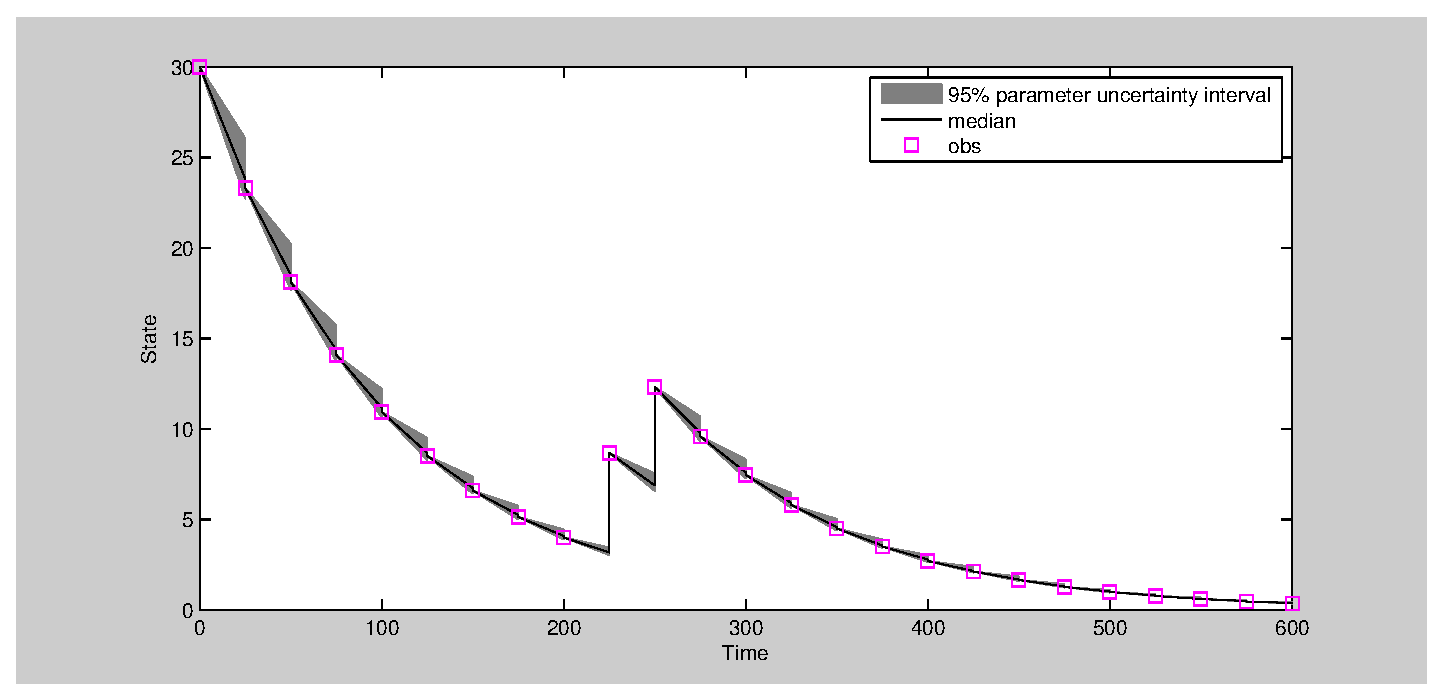
\includegraphics[width=\linewidth,keepaspectratio]{./../eps/result-of-patch-uncertainty-snippet-reset.eps}
  \caption{Result of running the code from Listing~\ref{list:patch-uncertainty-snippet-reset}.}
  \label{fig:result-of-patch-uncertainty-snippet-reset}
\end{figure}


%\section{MMSODA in reset mode; parallel execution}

%\smallq{Refer to Fig.~\ref{fig:mmsoda-workflow} in order to run the `example3' case on the LISA cluster.}

\section{MMSODA in `soda' mode; sequential execution}
\label{sec:soda-mode}
\index{MMSODA!soda mode}


\smallq{On your local machine, copy the `example3' directory to a new directory, `example4'. Clean up the `./results' subdirectory, and remove `matlabprog', `libmmpi.so', and `Makefile', as well as any jobscripts pertaining to `example3'.}

The `soda' mode is the most complex and most compute-intensive mode. It is similar to the `reset' mode in that it updates the model states during the simulation. The way the updating is performed, however, is different. The difference between `scemua', `reset', and `soda' modes essentially comes down to how much confidence is placed on the observed values of the state in comparison to how much confidence is placed on the simulated values of the state. For example, in `scemua' mode, all of the confidence is placed on the simulated values---the model can be run from the time of the initial state (\texttt{conf.priorTimes(1)}) to the time at which the last prediction is required (\texttt{conf.priorTimes(end)}), without the need for temporarily halting the model at \texttt{conf.priorTimes(2:end-1)} to do any state updating. In contrast to this, the `reset' mode places full condidence on the observations: at the times when an observation is available, the model is temporarily halted, and its states are reset to the value of the observed state. The `soda' mode then, provides sort of a middle ground between MMSODA's `scemua' and `reset' modes: instead of placing all of the confidence on one or the other, a little confidence is placed on both the simulated and the observed value of the states. A weighted average of the two is then calculated, and the simulated state (i.e.\,the prior state\index{prior state}\index{state!prior}) is adjusted in the direction of the observed state. The magnitude of the adjustment is sometimes referred to as the `state \textit{innovation}'\index{state!innovation} or simply `state \textit{update}'\index{state!update}. Adding the state update to the prior state results in a new state value, which is known as the `\textit{posterior} state'\index{posterior state}\index{state!posterior} or the `\textit{analysis} state'\index{analysis state}\index{state!analysis}.

%\textit{explanation of weighting prior state and obs if std or var are known. (i.e. normal Kalman Filter)\index{todo}}

%\textit{extend explanantion of weighting if the equations are not linear. the information is then stored by perturbing the prior and pertubing the obs, and then weighting them together.\index{todo}}

In terms of setup, the `soda' mode is not so different from the `reset' mode that you are familiar with. In fact, a quick look at the table of configuration variables in \texttt{mmsoda}'s documentation reveals that only 3 additional configuration variables are needed: \texttt{covObsPert}, \texttt{covModelPert}, and \texttt{nMembers}.

\smallq{Read the description in \texttt{mmsoda}'s documentation for these three options.}

\smallq{Include \texttt{covObsPert}, \texttt{covModelPert}, and \texttt{nMembers} in your `makeconf.m', and assign them values of \texttt{0.02}, \texttt{0.10} and \texttt{10}, respectively. Don't forget to change \texttt{modeStr} to \texttt{\squote{soda}}, otherwise MMSODA will overwrite the values of \texttt{covObsPert} and \texttt{covModelPert} with \texttt{0}. Set \texttt{nModelEvalsMax} to \texttt{150} for now, re-run `makeconf.m', and verify that `./results/conf.mat' was indeed written.}


\smallq{Re-read the documentation on the objective function (see Figure~\ref{fig:doc-the-objective-function}), in particular the description of the input argument \texttt{modelOutput}, which is 3-D if \texttt{modeStr} is \texttt{\squote{soda}}.}

\smallq{Adapt the objective function such that the SSR is calculated based on the ensemble-member mean of the prior state. Note: calculating the mean over the 3$\mathrm{^{rd}}$ dimension of an N-dimensional array \texttt{X} in MATLAB is easily achieved by \texttt{mu = mean(X,3)}.}

\smallq{Test your configuration locally until it works. Then set \texttt{nModelEvals} to \texttt{7000} and re-run `makeconf.m'.}

\smallq{Call \texttt{mmsodaPrepParallelFiles} to write the jobscript and the Makefile.}

\smallq{Copy your `example4' working directory to the cluster.}

%how does one determine the values of covobspert and covmodelpert?

\section{MMSODA in `soda' mode; parallel execution}

\smallq{Use PuTTY to set up an SSH connection to the LISA cluster. Make sure the necessary modules are loaded before compiling the binary. Submit your jobscript to the queue and wait for the optimization to finish.}

\smallq{Once the job finishes, edit `makeconf.m' on your local machine by setting \texttt{saveEnKFResults} to \texttt{true} and \texttt{startFromUniform} to \texttt{false}. Increase the maximum number of model evaluations by \texttt{500}. Run \texttt{makeconf} and copy the new MMSODA configuration to the remote system. Submit the jobscript to the queue once more, and wait for the results.}

\smallq{Copy the optimization results back to your local machine.}

\smallq{Copy the code snippet from Listing~\ref{list:patch-uncertainty-snippet-reset} to your working directory. Adapt the filename from which the optimization results are read, and run the snippet on the results of the `soda' mode optimization. The result should look like Fig.~\ref{fig:result-of-patch-uncertainty-snippet-soda}.}


\begin{figure}[htb]
  \centering
    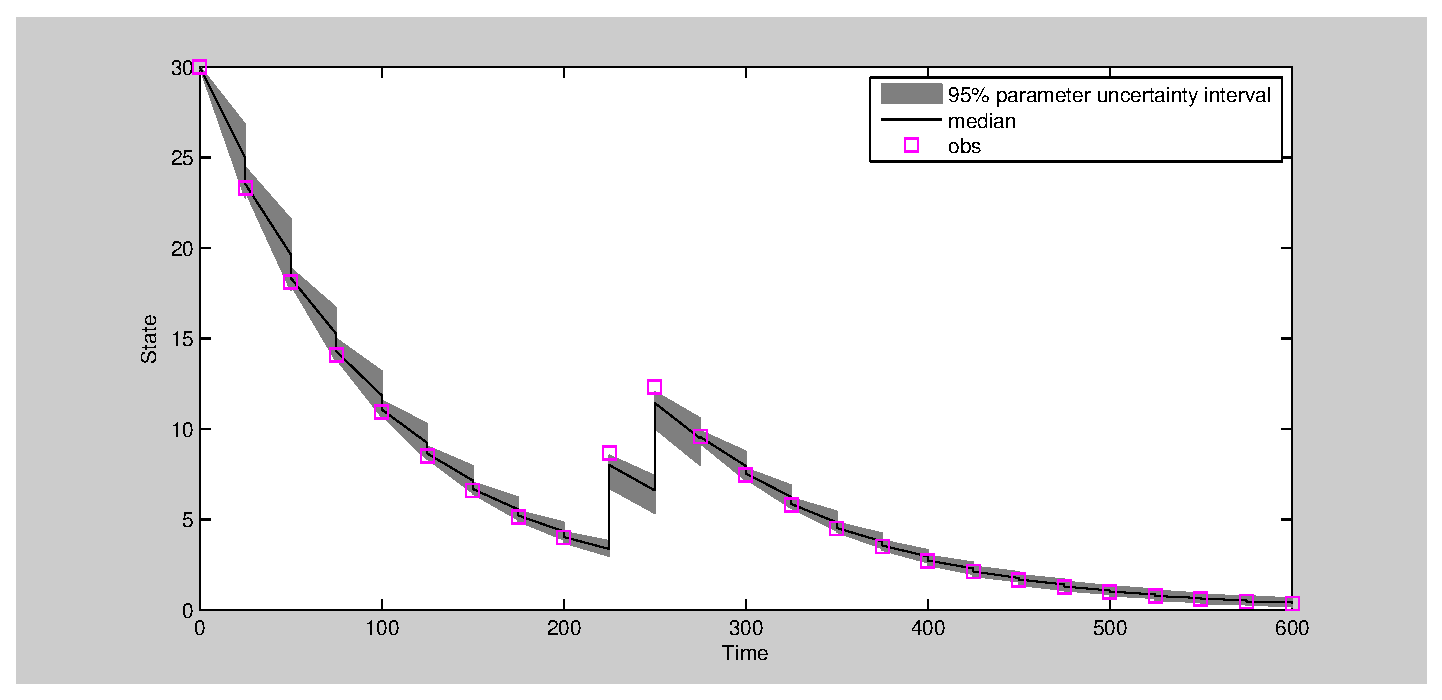
\includegraphics[width=\linewidth,keepaspectratio]{./../eps/result-of-patch-uncertainty-snippet-soda.eps}
  \caption{Parameter uncertainty intervals for the `soda' mode optimization of the lintank model.}
  \label{fig:result-of-patch-uncertainty-snippet-soda}
\end{figure}



